%%%%%%%%%%%%%%%%%%%%%%%%%%%%%%%%%%%%%%%%%
% Thesis Template Lab25 UNAM
% 
% (Thesis Template for the students of Lab25 at the UNAM)
% This Template was "fixed/built up" by Adriana Felisa Chávez (adrifelcha@gmail.com)
% as a mixture of two Previous Templates:

% 1) "unamthesis" originally developed by: Julio Augusto Freyre-González
% We took this template as a basis for desginging the front page
% (according to the requirements established by the UNAM)
%

% 2) 'Masters/Doctoral Thesis'  (Which is the basis for EVERYTHING else in this template)
% LaTeX Template
% Version 2.4 (22/11/16)
% Version 2.x major modifications by:
% Vel (vel@latextemplates.com)
% This template was based on a template by:
% Steve Gunn (http://users.ecs.soton.ac.uk/srg/softwaretools/document/templates/)
% Sunil Patel (http://www.sunilpatel.co.uk/thesis-template/)
% Which means...
% The second major version of the Masters/Doctoral Thesis template was made by Vel. 
% The thesis style was originally created by Steve R. Gunn and modified into a template by Sunil Patel.   
% Template license:
% CC BY-NC-SA 3.0 (http://creativecommons.org/licenses/by-nc-sa/3.0/)
% The rest of the Template (except the front page) was built according to this last Template


%Both of previously mentioned templates -used to build up the template you're using right now-
%can be downloaded from:
% http://www.LaTeXTemplates.com
%%%%%%%%%%%%%%%%%%%%%%%%%%%%%%%%%%%%%%%%%%

%----------------------------------------------------------------------------------------
%	PACKAGES AND OTHER DOCUMENT CONFIGURATIONS
%----------------------------------------------------------------------------------------

\documentclass[
12pt, % The font size (other options: 10pt, 11pt, 12pt)
%oneside, % Two side (alternating margins) for binding by default, uncomment to switch to one side
spanish, % language by default
singlespacing, % Single line spacing, alternatives: onehalfspacing or doublespacing
%draft, % Uncomment to enable draft mode (no pictures, no links, overfull hboxes indicated)
%nolistspacing, % If the document is onehalfspacing or doublespacing, uncomment this to set spacing in lists to single
%liststotoc, % Uncomment to add the list of figures/tables/etc to the table of contents
%toctotoc, % Uncomment to add the main table of contents to the table of contents
%parskip, % Uncomment to add space between paragraphs
%nohyperref, % Uncomment to not load the hyperref package
headsepline, % Uncomment to get a line under the header
%chapterinoneline, % Uncomment to place the chapter title next to the number on one line
%consistentlayout, % Uncomment to change the layout of the declaration, abstract and acknowledgements pages to match the default layout
]{Tesis_Lab25} % The class file specifying the document structure

\usepackage[utf8]{inputenc} % Required for international characters
\usepackage[T1]{fontenc} % Output font encoding for international characters
\usepackage{graphics}
\usepackage{utopia} % Dr. Bouzas is confortable with this font; but you may preffer using Palatino
\usepackage[spanish]{babel}
\usepackage[latin1]{inputenc}
%\usepackage{arial}
\usepackage[backend=bibtex,style=authoryear,natbib=true]{biblatex} % Use the bibtex backend with the authoryear citation style (which resembles APA)
%\usepackage[natbibapa]{apacite}
%\bibliographystyle{apacite}

\addbibresource{Bib_Jaime.bib} % The filename of the bibliography

%\usepackage[autostyle=true]{csquotes} % Required to generate language-dependent quotes in the bibliography

%----------------------------------------------------------------------------------------
%	MARGIN SETTINGS
%----------------------------------------------------------------------------------------

\geometry{
	paper=a4paper, % Change to letterpaper for US letter
	inner=2.5cm, % Inner margin
	outer=3.8cm, % Outer margin
	bindingoffset=.5cm, % Binding offset
	top=1.5cm, % Top margin
	bottom=1.5cm, % Bottom margin
	%showframe, % Uncomment to show how the type block is set on the page
}

%----------------------------------------------------------------------------------------
%	THESIS INFORMATION
%----------------------------------------------------------------------------------------

\thesistitle{Niveles Cognitivos y Creencias en Juegos} % Your thesis title, print it with \ttitle
\supervisor{Dr. Arturo Bouzas Riaño} % Your supervisor's name, print it with \supname
\examiner{Dr. Óscar Zamora Arévalo} % Your examiner's name, print it with \examname
\degree{Licenciatura en Psicología} % Your degree name, print it with \degreename
\author{Jaime Osvaldo Islas Farías}% Your name, print it with \authorname

\subject{Psicología} % Your subject area, print it with \subjectname
\keywords{} % Keywords for your thesis, print it with \keywordnames
\university{\href{http://www.university.com}{Universidad Nacional Autónoma de México}} % Your university's name and URL, print it with \univname
\department{\href{http://department.university.com}{Laboratorio de Comportamiento Adaptable}} % Your department's name and URL, print it with \deptname
\group{\href{http://researchgroup.university.com}{Laboratorio de Comportamiento Adaptable}} % Your research group's name and URL, print it with \groupname
\faculty{\href{http://faculty.university.com}{Facultad de Psicología}} % Your faculty's name and URL, print it with \facname

\sinodalA{Sinodal 1} % The name of your 1st Sinodal; print it with \SinodalA
\sinodalB{Sinodal 2} % The name of your 2nd Sinodal; print it with \SinodalB
\sinodalC{Sinodal 3} % The name of your 3rd Sinodal; print it with \SinodalC

\city{Ciudad de México} % Your city; print it with \city

\proyectopapime{PAPIME PE310016}   % The 1st project from where you received financial support, print it with \PAPIIT
\proyectopapiit{PAPIIT IN307214}   % The 2nd project from where you received financial support, print it with \PAPIME

\AtBeginDocument{
\hypersetup{pdftitle=\ttitle} % Set the PDF's title to your title
\hypersetup{pdfauthor=\authorname} % Set the PDF's author to your name
\hypersetup{pdfkeywords=\keywordnames} % Set the PDF's keywords to your keywords
}

%----------------------------------------------------------------------------------------
%	LET THE THESIS BEGIN!
%----------------------------------------------------------------------------------------

\begin{document}

\frontmatter % With this, you use roman page numbering style (i, ii, iii, iv...) for the pre-content pages

\pagestyle{plain} % Default to the plain heading style until the thesis style is called for the body content

%----------------------------------------------------------------------------------------
%	FRONT PAGE (According to the UNAM requirements)
%----------------------------------------------------------------------------------------

\begin{titlepage}
\begin{minipage}[c][9in][s]{1in}
\centering
\hspace*{-0.2in} 
\includegraphics[width=1.1in]{Escudo-UNAM}\\[10pt]
\hskip 2pt\vrule width 2pt height 6.7in
\hskip 1mm\vrule width 1pt height 6.7in\\[10pt]
\hspace*{-0.2in} 
\includegraphics[width=1.2in]{PSI}
\end{minipage}\hskip 10pt
% Right layout - Titles
\begin{minipage}[c][\textheight][s]{5.125in}
\centering
% University, institute, department and title
{\Large\scshape\univname}
\vspace{3mm}\hrule height2pt
\vspace{1mm}\hrule height1pt
\vspace{3mm}
{\scshape\facname}\par
% Title
\vfill\vfill
{\def\baselinestretch{1}\LARGE\scshape\ttitle\par}
\vfill\vfill
% Degree, author, supervisor and date
\makebox[8cm][s]{\Huge T E S I S}\\[8pt]
QUE PARA OBTENER EL GRADO DE:\\[8pt]
{\scshape\degreename}\\[16pt]
{\huge P  R  E  S  E  N  T  A:}\\[8pt]
{\large {\scshape\authorname}}\par
\vfill
{\small DIRECTOR DE TESIS:\\{\scshape\supname}}\par
\vfill
{\small REVISOR:\\{\scshape\examname}}\par
\vfill
{\small SINODALES:\\{\scshape\SinodalA}}\\{\scshape\SinodalB}}\\{\scshape\SinodalC}}\par
\vfill
{\small Con el apoyo de:\\Proyecto {\scshape\PAPIIT}}\par   
%If you only received financial support from a single project, you may delete "y \\Proyecto {\scshape\PAPIME}"
\vfill
{\hspace{0.2in}\scshape\city\hfill\today}
\end{minipage}
\end{titlepage}
\begin{titlepage}
\centering\large
{\def\baselinestretch{1.2}\Large\bfseries\ttitle\par}\\
\vspace{15mm}
por\par
\vspace{15mm}
{\Large\authorname}
\vspace{40mm}
\par
Tesis presentada para obtener la\par
\vspace{15mm}
\degreename\par
\vspace{15mm}
en la\par 
\vspace{15mm}
\facname
\par
\vspace{15mm}
{\Large\scshape\univname}
\vspace{30mm}
\par
\city, \today
\end{titlepage}}



%----------------------------------------------------------------------------------------
%	DECLARATION PAGE
%----------------------------------------------------------------------------------------

\begin{declaration}
\addchaptertocentry{\authorshipname} % Add the declaration to the table of contents
\noindent Yo, \authorname, declaro que la tesis aquí presentada bajo el título \enquote{\ttitle}, es de mi entera autoría. Aclarando que:\\

\begin{itemize} 
\item La presente tesis fue trabajada en el Laboratorio 25 de la Facultad de Psicología de la Universidad Nacional Autónoma de México, bajo la tutela del Dr. Arturo Bouzas Riaño. 
\item Ningún dato aquí presentado ha sido utilizado con anterioridad para recibir un grado académico ni en ésta ni en ninguna otra Universidad. 
\item Las ideas cuya autoría no me corresponde retomadas en el texto, están clara y adecuadamente señaladas. Toda cita se señala y vincula a la fuente de donde se obtuvo. Con excepción de dichos fragmentos citados, todo lo aquí escrito es enteramente mi responsabilidad, producto de mi trabajo. 
\item Todas las figuras aquí presentadas fueron elaboradas en RStudio (lenguaje R) y Spyder (lenguaje Python) por la autora de la presente tesis, a menos que se señale lo contrario.
\item He señalado y dado crédito a todas las posibles fuentes de apoyo consultadas (lenguajes de programación, códigos base y manuales varios).
%\item Cualquier porción del trabajo aquí expuesto que se haya realizado en colaboración directa o indirecta con un tercero, es señalada y presentada con claridad.
\item El presente proyecto de investigación fue realizado con el apoyo de PAPIIT IN307214 y PAPIME PE310016.\\
\end{itemize}
 
\noindent Firma:\\
\rule[0.5em]{25em}{0.5pt} % This prints a line for the signature
 
\noindent Fecha:\\
\rule[0.5em]{25em}{0.5pt} % This prints a line to write the date
\end{declaration}

\cleardoublepage

%----------------------------------------------------------------------------------------
%	QUOTATION PAGE
%----------------------------------------------------------------------------------------

\vspace*{0.2\textheight}

\noindent\enquote{\itshape Aquí pueden poner una cita super padriurix.}\bigbreak

%My experiences with science led me to God. They challenge science to prove the existence of God. But must we really light a candle to see the sun?
%1972

%Read more at: https://www.brainyquote.com/quotes/authors/s/steven_pinker_2.html
\hfill Autor de la cita, año.\\\\\\\\\\\\\\\\\\\\\\\\\\\\\\\\




%----------------------------------------------------------------------------------------
%	ABSTRACT PAGE
%----------------------------------------------------------------------------------------

\begin{abstract}
\addchaptertocentry{\abstractname} % Add the abstract to the table of contents

En esta página va a ir el resumen de tu trabajo. En esta página va a ir el resumen de tu trabajo. En esta página va a ir el resumen de tu trabajo. En esta página va a ir el resumen de tu trabajo. En esta página va a ir el resumen de tu trabajo. En esta página va a ir el resumen de tu trabajo. En esta página va a ir el resumen de tu trabajo . En esta página va a ir el resumen de tu trabajo . En esta página va a ir el resumen de tu trabajo .En esta página va a ir el resumen de tu trabajo .En esta página va a ir el resumen de tu trabajo. En esta página va a ir el resumen de tu trabajo . En esta página va a ir el resumen de tu trabajo . En esta página va a ir el resumen de tu trabajo . En esta página va a ir el resumen de tu trabajo . En esta página va a ir el resumen de tu trabajo . En esta página va a ir el resumen de tu trabajo . En esta página va a ir el resumen de tu trabajo . En esta página va a ir el resumen de tu trabajo\\

\end{abstract}

%\ldots
%----------------------------------------------------------------------------------------
%	ACKNOWLEDGEMENTS
%----------------------------------------------------------------------------------------

\begin{acknowledgements}
\addchaptertocentry{\acknowledgementname} % Add the acknowledgements to the table of contents

Aquí van los nombres de las personas que sean dueñas de sus bellos corazones.\\

Aquí van los nombres de las personas que sean dueñas de sus bellos corazones.\\

Aquí van los nombres de las personas que sean dueñas de sus bellos corazones.\\

Aquí van los nombres de las personas que sean dueñas de sus bellos corazones.\\

Aquí van los nombres de las personas que sean dueñas de sus bellos corazones.\\

Aquí van los nombres de las personas que sean dueñas de sus bellos corazones.\\

Aquí van los nombres de las personas que sean dueñas de sus bellos corazones.\\

Aquí van los nombres de las personas que sean dueñas de sus bellos corazones.\\

Aquí van los nombres de las personas que sean dueñas de sus bellos corazones.\\

Aquí van los nombres de las personas que sean dueñas de sus bellos corazones.\\

\end{acknowledgements}

%----------------------------------------------------------------------------------------
%	LIST OF CONTENTS/FIGURES/TABLES PAGES
%----------------------------------------------------------------------------------------

\tableofcontents % Prints the main table of contents

\listoffigures % Prints the list of figures

\listoftables % Prints the list of tables

%----------------------------------------------------------------------------------------
%	ABBREVIATIONS
%----------------------------------------------------------------------------------------

\begin{abbreviations}{ll} % Include a list of abbreviations (a table of two columns)

\textbf{BTW} & \textbf{B}y-\textbf{T}he \textbf{W}ay\\
\textbf{LOL} & \textbf{L}aughing \textbf{O}ut \textbf{L}oud\\
\textbf{ROFL} & \textbf{R}olling \textbf{O}n \textbf{F}loor \textbf{L}aughing\\

\end{abbreviations}

%----------------------------------------------------------------------------------------
%	DEDICATION
%----------------------------------------------------------------------------------------

\dedicatory{En memoria de la buena Felisa\ldots} 

%----------------------------------------------------------------------------------------
%	THESIS CONTENT - CHAPTERS
%----------------------------------------------------------------------------------------

\mainmatter % Begin numeric (1,2,3...) page numbering

\pagestyle{thesis} % Return the page headers back to the "thesis" style

% Include the chapters of the thesis as separate files from the Chapters folder

% Chapter 1

\chapter{Introducción} % Main chapter title

\label{Chapter1} % For referencing the chapter elsewhere, use \ref{Chapter1} 

%----------------------------------------------------------------------------------------

% Define some commands to keep the formatting separated from the content 
\newcommand{\keyword}[1]{\textbf{#1}}
\newcommand{\tabhead}[1]{\textbf{#1}}
\newcommand{\code}[1]{\texttt{#1}}
\newcommand{\file}[1]{\texttt{\bfseries#1}}
\newcommand{\option}[1]{\texttt{\itshape#1}}

%----------------------------------------------------------------------------------------

Teoría de juegos es una rama de las matemáticas que estudia la toma de decisiones en situaciones de interacción. Dentro de teoría de juegos, se estudian situaciones como la que representa el juego del ciempiés (estudiada por primera vez por Rosenthal, en 1982). Se trata de un juego donde dos jugadores, A y B, toman turnos para elegir si quedarse con una ganancia acumulada o pasar la ganancia al otro jugador. Si algún jugador elige quedarse con la ganancia acumulada, el otro jugador no recibe nada y el juego termina. En cambio, si el jugador elige pasar, el tamaño de la ganancia acumulada aumenta. El juego dura 10 turnos, y la ganancia acumulada aumenta su valor en cada uno. Si en el último turno, que le corresponde al jugador B, este elige pasar, el jugador A se queda con todas las ganancias.\\

De acuerdo con las reglas del juego, si los jugadores quisieran maximizar sus ganancias, deberían elegir ‘pasar’ para que la ganancia acumulada siga aumentando, pero al mismo tiempo, dado que ambos jugadores quieren quedarse con la ganancia, deben elegir quedarse con ella antes de que lo haga el otro jugador. ¿En qué turno del juego sería una buena elección (para cada jugador) quedarse con la ganancia acumulada?\\

El juego establece que en el último turno, cuando la ganancia acumulada tiene su valor más alto, le corresponde elegir al jugador B. Si este jugador elige pasar, todas las ganancias serán para el jugador A, mientras que si decide quedarse con la ganancia acumulada, B obtendrá la mayor ganancia posible. Por lo tanto, el jugador B debería elegir quedarse con la ganancia en el turno 10. Sin embargo, este razonamiento no es un secreto para el jugador A. Si el jugador A sabe que al jugador B le conviene quedarse con la ganancia en el turno 10 (en cuyo caso A se quedaría sin nada), entonces la mejor estrategia para el jugador A consiste en quedarse con la ganancia acumulada en el turno 9. Pero así como el jugador A es capaz de anticipar que el jugador B elegirá quedarse con la ganancia en el turno 10, el jugador B puede deducir que el jugador A elegirá quedarse con la ganancia en el turno 9. Si este es el caso, el jugador B debería elegir quedarse con la ganancia en el turno 8. Si ambos jugadores repiten este razonamiento para todos los turnos de juego, eventualmente se llega a la conclusión de que la mejor estrategia para cualquiera de los jugadores en cualquier turno es elegir quedarse con la ganancia, sin importar el turno en que se encuentren. A este proceso de repetir un razonamiento para llegar a la mejor estrategia disponible tomando en cuenta que el otro jugador también puede hacerlo, se conoce como razonamiento iterado, y es uno de los conceptos básicos en teoría de juegos.\\

A las situaciones donde los jugadores eligen la estrategia que maximice su ganancia esperada, tomando en cuenta las estrategias de los otros jugadores, se les conoce como el equilibrio de Nash, otro concepto básico en teoría de juegos. En el juego del ciempiés, el equilibrio de Nash supondría que el jugador A se quede con la ganancia acumulada desde el primer turno del juego, incluso si en este punto su valor es muy pequeño.\\

En muchas situaciones de interacción, el razonamiento requerido para llegar al equilibrio es demasiado complejo para ser plausible en términos conductuales, por lo que cuando personas reales se encuentran en dicho tipo de situaciones, sus elecciones suelen ser distintas de lo que supondría el equilibrio. Sin embargo, existe evidencia de que el aprendizaje (jugar un juego de forma repetida) genera una tendencia a converger al equilibrio y solo en situaciones donde no se permite que haya aprendizaje, se puede atribuir el equilibrio al pensamiento estratégico por sí sólo (Crawford, Costa-Gomes & Iriberri, 2013).
El equilibrio se ve reflejado tanto en las elecciones de los participantes del juego, como en sus creencias sobre los otros participantes: jugadores que son racionales (en términos de teoría de decisión) tienen creencias correctas sobre los otros jugadores, si estos también son racionales (Crawford, Costa-Gomes & Iriberri, 2013).\\

Durante el proceso de razonamiento iterado, los jugadores incorporan las creencias que tienen sobre la conducta de los otros jugadores en su toma de decisiones. Keynes (1936) ilustró el proceso de razonamiento iterado con una analogía que se conoce como Beauty contest: Un concurso en el que los participantes deben elegir de entre cien fotografías de rostros, cuáles piensan que los demás participantes considerarán que son los más atractivos. Tomando en cuenta que todos los participantes se enfrentan al mismo problema, para ganar no basta con elegir solamente aquellos rostros que piensen que son los más atractivos, o cuáles piensan que los demás participantes piensan que son más atractivos, sino aquellos que piensen que los demás participantes pensarán que los demás participantes piensan que son los más atractivos. Esto implica tres pasos de razonamiento iterado.\\

Un agente totalmente racional debería realizar tantos pasos de razonamiento iterado como fueran necesarios para llegar a la solución por dominancia del juego (el equilibrio de Nash). En la realidad, las personas no se comportan de forma perfectamente racional, y la cantidad de pasos de razonamiento iterado que realizan es limitada (Stahl & Wilson, 1995, Ho, Caremer & Weigelt, 1998).
Experimentalmente el juego p-Beauty contest, llamado así a partir de la analogía de Keynes, ha sido utilizado para estudiar el razonamiento iterado. En este juego, en el que participan varios participantes (por lo menos 3), cada uno debe elegir un número entero en el rango [0 - 100], de manera simultánea y sin revelarlo a los otros jugadores. Posteriormente, se calcula la media de todos los números elegidos y este valor se multiplica por un parámetro p que es un número positivo y diferente de 1, conocido de antemano por todos los jugadores, (generalmente se utiliza p = 2/3). Al valor resultante de este cálculo se le llama el número objetivo, y el ganador del juego será el participante que haya elegido el número más cercano a este número.\\

Si los jugadores fueran perfectamente racionales, creyeran que los demás jugadores también lo son y además pudieran realizar una cantidad infinita de pasos de razonamiento iterado, llegarían a la solución por dominancia del juego mediante el siguiente razonamiento: El valor más grande que puede alcanzar el número objetivo (con p = 2/3) es 100× p=66.66, así que cualquier número arriba de este valor es dominado por 66.66. Jugadores racionales obedecerán la dominancia y creerán que los demás jugadores lo harán también, por lo que todos elegirán un número menor a 66.66. Por lo tanto, el valor máximo del número objetivo será 100×p^2=44.44 y elegir cualquier número por arriba de este será una estrategia dominada. Aplicando este razonamiento una y otra vez (de ahí el nombre de razonamiento iterado), el valor del número objetivo se reduce con cada iteración, hasta que se llega al equilibrio de Nash del juego, que todos los jugadores elijan 0 (Nagel, 1995; Ho, Camerer, Weigelt, 1998).\\

Empíricamente, esto no suele ocurrir, pero cuando el mismo grupo de participantes juegan repetidamente (más de un periodo), se ha reportado consistentemente que sus elecciones se acercan paulatinamente al equilibrio (elegir 0) con cada periodo (Nagel, 1995, Ho, Camerer & Weigelt, 1998). También se ha observado que dicha tendencia se interrumpe cuando se agregan nuevos participantes al juego, siendo que los jugadores con experiencia incrementan el número elegido al enfrentarse a estos jugadores novatos, lo que se conoce como efecto de reset (Slonim, 2005).\\

Se han propuesto varios modelos que dan cuenta de la forma en la que las personas eligen sus números en el juego. Estos modelos capturan la noción de que la elección de las personas es un reflejo del número de pasos de razonamiento iterado que son capaces de realizar, que en la literatura de juegos se conoce como “nivel cognitivo”, así como de las creencias o expectativas que tienen sobre el nivel cognitivo de los demás jugadores (Crawford, Costa-Gomes & Iriberri, 2013).\\

Algunos estudios (Agranov et al., 2012 y Slonim, 2005)  han explorado el efecto que tienen las creencias sobre el desempeño de los otros jugadores en las elecciones de cada participante, evaluando esta relación de forma indirecta y encontrando evidencia a favor de una relación positiva. En contraste, en otros estudios que han intentado tener un acercamiento más directo, se han encontrado inconsistencias entre las creencias sobre lo que harán los otros jugadores y las elecciones reales; Lahav (2015) utilizó un método en el que le pidió a los jugadores hacer una estimación indirecta de las elecciones de los otros jugadores y comparó directamente estas creencias con sus elecciones reales, encontrando una falta de consistencia entre las dos.\\

El presente trabajo de investigación pretende estudiar de manera directa la relación entre las elecciones de las personas y sus creencias sobre las elecciones de los demás, y adicionalmente explora si la experiencia que se adquiere jugando el juego de forma repetida influye en la relación de estas dos variables.\\

El diseño experimental consiste en juegos repetidos de p-beauty contest (estructurados en 2 subjuegos compuestos por 4 periodos cada uno). En cada sesión experimental, un solo jugador participa en el juego durante los dos subjuegos, siendo que al término del Subjuego 1 los demás jugadores son reemplazados por nuevos participantes que no han jugado previamente. Además de registrar los números elegidos por cada participante en cada periodo, se les solicita a los jugadores que reporten directamente los números que creen que los demás elegirán. Este método de explicitar creencias permite comparar directamente las elecciones y las creencias de los jugadores, de forma más evidente a la utilizada por Lahav (2015), si bien igual que en ese estudio, acercarse a los números que eligen los otros jugadores es recompensado con ganancias en el juego para agregar motivación a la expresión de las creencias.
Se encontró que la entrada de nuevos jugadores en el segundo subjuego incrementa el número elegido de los jugadores con experiencia en el primer periodo de este nuevo subjuego, pero la diferencia entre sus creencias y elecciones no incrementa junto con esta, lo que aporta evidencia de que la adquisición de experiencia incrementa la consistencia.\\

El resto de la tesis está dividida en cinco apartados: En el primero se presenta el marco teórico, que describe el modelo de nivel-k usado para explicar la conducta de las personas en el juego. La sección también revisa la relación empírica entre las elecciones de las personas y sus creencias, y la forma en que la experiencia en juegos repetidos influye en las elecciones de los jugadores. También se detallan los objetivos concretos del trabajo de investigación y las estrategias para alcanzarlos. En el segundo apartado se describe el método utilizado, incluyendo información sobre los participantes, el procedimiento y el diseño experimental. En el tercer apartado se presentan los resultados del experimento. Se reporta el grado de consistencia que existe entre creencias y elecciones de los jugadores en el primer subjuego, el efecto de introducir a participantes sin experiencia en el segundo subjuego, y las diferencias en consistencia entre creencias y elecciones que hay entre los dos subjuegos. Por último, en el cuarto apartado se elabora la discusión a partir de los resultados, y las conclusiones se presentan en el quinto apartado.\\

% Chapter 1
\chapter{Marco Teórico} % Main chapter title

\label{Cap_SDT} % For referencing the chapter elsewhere, use \ref{Chapter1} 

%----------------------------------------------------------------------------------------

% Define some commands to keep the formatting separated from the content 
\newcommand{\keyword}[1]{\textbf{#1}}
\newcommand{\tabhead}[1]{\textbf{#1}}
\newcommand{\code}[1]{\texttt{#1}}
\newcommand{\file}[1]{\texttt{\bfseries#1}}
\newcommand{\option}[1]{\texttt{\itshape#1}}

%----------------------------------------------------------------------------------------

\section{Modelo de nivel-k}

Este modelo fue propuesto por Nagel, (\citeyear{Nagel}), para dar cuenta de la conducta de las personas en juegos con solución por dominancia, como ocurre con textit{p-beauty contest}. El modelo define niveles cognitivos que describen el número de pasos de razonamiento iterado que realiza una persona en el juego y difiere respecto de los modelos de equilibrio clásicos, en que las creencias que se tienen sobre las elecciones de los otros jugadores no están basadas en la definición del equilibrio (Nash, \citeyear{Nash}, Crawford, Costa-Gomes & Iriberri, \citeyear{Crawford}), es decir, admite la posibilidad de que los otros jugadores no son perfectamente racionales.\\ 

Según este modelo, los jugadores con un nivel cognitivo 0 serían aquellos que no realizan ningún paso de razonamiento iterado, es decir, que no toman en consideración que las elecciones de los otros participantes influyen en el cálculo del número objetivo. Estos jugadores eligen un número con base en alguna regla arbitraria, (por ejemplo, su número de la suerte o favorito), por lo que podrían elegir cualquier número dentro del rango establecido con una probabilidad similar.\\

Un jugador de nivel 1 es aquel que sí considera que las elecciones de los otros jugadores influyen en el cálculo del número objetivo, pero supone que los otros jugadores no han tomado esto en consideración. El jugador de nivel 1 asume que los demás jugadores son de nivel 0 y elige el número que es la respuesta óptima contra este tipo de jugadores, asumiendo que la media de los números elegidos por todos los jugadores estará cerca de 50 (el mejor predictor de la media de un conjunto de números aleatorios en el rango [0 - 100]) y multiplicará este número por $p$ para acercarse lo más posible al número objetivo.\\

Por su parte, un jugador de nivel 2 no sólo considera que las elecciones de otros jugadores influyen en el número objetivo, sino que también asume que los otros jugadores saben esto. El jugador de nivel 2 elegirá el número que es la respuesta óptima contra una población de oponentes de nivel 1, y como éstos eligen números cercanos a $50 \cdot p$, el jugador de nivel 2 debe multiplicar por $p$ nuevamente para acercarse al que piensa que será el número objetivo, esto es $50 \cdot p^2$.\\

En general, un jugador de nivel $k$ elegirá la respuesta óptima contra una población de jugadores de nivel $k-1$, esto es $50 \cdot p^k$.  Con base en esta regla, el modelo computa el nivel cognitivo de los jugadores en función de a cuál de los intervalos de elección establecidos por el modelo pertenece su número elegido.\\

Una variación más sofisticada del modelo de nivel-k es el modelo de jerarquía cognitiva, propuesto por Camerer, Ho, y Chong, (\citeyear{Camerer}). El modelo propone que un jugador de nivel $k$ no sólo da la mejor respuesta contra jugadores $k-1$, sino a una combinación de todos los tipos de jugador desde el nivel 0 hasta $k-1$, a partir de una distribución Poisson que se actualiza de forma bayesiana. El modelo mantiene el supuesto de que las personas consideran que su nivel está por arriba de los demás jugadores, y predice un aprendizaje sobre los niveles $k$ de los otros jugadores.\\

En general, de acuerdo con la evidencia obtenida experimentalmente, los modelos de nivel-k explican mejor el comportamiento de las personas en juegos con solución por razonamiento iterado que los modelos de equilibrio (Crawford, Costa-Gomes & Iriberri, \citeyear{Crawford}).\\

En los dos modelos previamente descritos, la elección de los jugadores depende de tres elementos: 1) sus creencias sobre cómo juegan los participantes de nivel 0; 2) sus expectativas sobre el nivel cognitivo de los oponentes; y 3) el número de pasos de razonamiento que son capaces de hacer en el juego (Agranov et al., \citeyear{Agranov}).\\

En la siguiente sección se ahonda sobre el segundo elemento: las expectativas (textit{i. e. creencias} sobre el nivel cognitivo de sus oponentes, y la evidencia que se ha encontrado sobre su relación con la elección.\\

\section{Relación entre creencias y elecciones}

Para aportar evidencia empírica de la influencia de las creencias acerca de la sofisticación de los otros jugadores sobre las elecciones de los jugadores en p-beauty contest, Agranov et al. (\citeyear{Agranov}), manipularon las creencias que los participantes tenían sobre sus oponentes, informando a cada participante que jugaría contra siete estudiantes graduados de Economía con conocimiento sobre este tipo de juegos, o bien, contra siete computadoras programadas para seleccionar aleatoriamente, con la misma probabilidad,  números dentro del rango [0 – 100]. En este estudio se encontró que los números registrados por los participantes corresponden con un nivel cognitivo significativamente mayor cuando se les decía que se enfrentarían a estudiantes graduados que cuando creían competir contra las computadoras. Este resultado parece sugerir que el nivel cognitivo que muestran las personas en juegos de p-beauty contest depende no únicamente de su sofisticación cognitiva, sino también de sus creencias sobre la sofisticación de los otros jugadores.\\

Para estudiar de forma más directa la relación entre las creencias y las elecciones de los participantes, Lahav (\citeyear{Lahav}) utilizó un método con \textit{elicited beliefs} (la mejor forma de traducirlo sería “\textit{que hace explícitas las creencias}”) en sesiones experimentales compuestas por 5 periodos de p-beauty contest con hasta 20 participantes. En cada periodo, además de elegir su propio número, se les pidió a los participantes que estimaran cuántos de los otros participantes elegirían un número dentro de cada uno de 10 posibles intervalos en el rango $0-100$ ($0-10$, $11-20$, $21-30$, …, $91-100$) y con dichas estimaciones, se calcularon las creencias de los participantes sobre el número promedio en cada periodo del juego. Al implementar este método, en contraste con investigaciones previas, Lahav concluye que las elecciones no son un reflejo preciso de las creencias de los participantes, pues encuentra diferencias significativas entre el número objetivo computado de acuerdo a las creencias de los participantes acerca de las tiradas de los demás jugadores y el número que de hecho eligen en el juego.\\

Otra investigación con resultados similares fue realizada por Costa-Gomes y Weizsäcker en el \citeyear{Costa-Gomes}, utilizando un método para explicitar creencias en juegos sencillos de 3x3 (donde dos jugadores tienen que elegir entre tres estrategias posibles), en los que es posible llegar al equilibrio del juego mediante razonamiento iterado. En dicha investigación se encontró que en la mayoría de los casos, de acuerdo con el modelo de nivel-k, las creencias registradas por los jugadores acerca de sus oponentes los situaban en el nivel 2, mientras que sus elecciones correspondían al nivel 1. Ya que no parece que las elecciones observadas habrían sido una respuesta óptima ante las creencias explicitadas que se registraron, este resultado pone en duda que estas últimas sean la base a partir de la cual los participantes emiten sus respuestas. A la luz de estos hallazgos, los autores concluyen que los jugadores basan sus decisiones en reglas de elección que influyen en ambas, creencias y decisiones.\\

Debido a que el presente trabajo de tesis incorpora parte del método de Lahav (\citeyear{Lahav}) para recopilar las creencias de los jugadores acerca de las tiradas de sus oponentes en juegos de p-beauty contest, se enfatizan los siguientes puntos respecto del estudio citado: \\

\begin{enumerate}
\item El método propuesto no permite conocer con exactitud la creencia de los participantes sobre el número objetivo. En su lugar, se obtuvo un cálculo aproximado de esta a partir del número de jugadores que se creyó elegirían un número dentro de cada intervalo, tomando la media de cada intervalo como valor de referencia.\\

\item Con alrededor de 20 personas participando en el juego, parece inverosímil, dada la demanda cognitiva, que los jugadores puedan calcular con precisión el número objetivo derivado de sus creencias acerca de las elecciones del resto de los participantes para emitir su respuesta.\\

\item Se contó con dos grupos control. En uno, no se realizó la explicitación de creencias, y en el otro, dicho procedimiento se realizó después de que los participantes hubieran eligido su número. Comparado la elección de los participantes en los grupos control con el grupo experimental, los resultados indican que solicitar a los participantes que registraran sus creencias no cambia significativamente  su número elegido.\\

\item El último periodo del juego fue el único en el que no se encontraron diferencias significativas entre creencias y elecciones, lo que podría sugerir que dicha discrepancia disminuye con la experiencia.\\

\item Dado que se sabe que los participantes tienden a elegir números cada vez más pequeños en cada periodo y que esto reduce invariablemente la magnitud de cualquier diferencia entre elecciones y creencias (ya que las diferencias entre números más pequeños son, por definición, más pequeñas), Lahav implementó un método de normalización con el que ponderó las diferencias entre las creencias y elecciones de cada participante en cada periodo por el promedio de los números elegidos por todos los participantes en dicho periodo. Sin embargo, como la medida de normalización depende de la tirada de todos los jugadores, la magnitud de la diferencia normalizada es afectada por el nivel cognitivo promedio, y “castiga” (incrementa la magnitud) las diferencias entre creencias y elecciones cuando estas no son tan sofisticadas como las del promedio. Debido a esto, podría no ser la mejor forma de compensar la tendencia al equilibrio.\\
\end{enumerate}

El resultado mencionado en el punto 4 permite cuestionar si la discrepancia entre creencias y elecciones se ve afectada por la experiencia que tienen los participantes en el juego.  En la siguiente sección se revisa el efecto de la experiencia en juegos repetidos de p-beauty contest.\\

\section{El efecto de la experiencia}

Para estudiar el efecto de la experiencia en juegos repetidos de p-beauty contest, Slonim (\citeyear{Slonim}) realizó sesiones experimentales de 12 periodos, distribuidos equitativamente en tres subjuegos con tres jugadores.\\

En una primera condición, al terminar cada subjuego se reemplazaba a dos de los tres participantes por jugadores nuevos, siendo que sólo un jugador permanecía en el experimento durante los 12 periodos completos. En una segunda condición, los dos participantes retirados al término de cada subjuego eran sustituidos por jugadores con la misma experiencia que el jugador que se mantenía en el juego (es decir, que habían jugado la misma cantidad de periodos). En ambas condiciones, los participantes tenían información acerca del nivel de experiencia de los demás jugadores (el número de periodos jugados).\\

Slonim (\citeyear{Slonim}) reportó que en el primer periodo de los subjuegos 2 y 3, los jugadores con más experiencia mostraron un mayor nivel cognitivo (es decir, eligieron números más cercanos a 0) cuando sabían que jugaban contra oponentes con la misma experiencia que ellos, que cuando jugaban contra oponentes que no habían jugado previamente. Este resultado aporta evidencia a favor de que las creencias sobre el nivel cognitivo de los otros jugadores influyen en las elecciones individuales. Por su parte, los jugadores sin experiencia no mostraron diferencias significativas en sus elecciones cuando jugaron con oponentes experimentados o no experimentados.\\

En cuanto al efecto de la experiencia en el desempeño de los jugadores, también se observó que los jugadores experimentados ganan el juego con mayor frecuencia cuando juegan con jugadores sin experiencia, ventaja que se reduce periodo a periodo, conforme los otros jugadores adquieren experiencia.\\

Un último resultado reportado por Slonim (\citeyear{Slonim}), y probablemente el de mayor relevancia para efectos de la presente tesis, corresponde a un efecto de reset en la tendencia a ir reduciendo el número elegido en cada periodo, al iniciar un nuevo subjuego. Es decir, que los jugadores con experiencia presentan una reversión en la tendencia a elegir números cada vez más cercanos al equilibrio cuando nuevos jugadores entran en el juego.\\

Con base en estos hallazgos, y los reportados en las secciones anteriores, se procede a plantear formalmente el objetivo de este trabajo de investigación, así como las estrategias metodológicas empleadas para llevarlo a cabo. \\

\section{Objetivo}

El presente trabajo de investigación busca evaluar si la reducción en las diferencias entre las creencias y elecciones, reportada con un método de explicitación de creencias similar al propuesto por Lahav (\citeyear{Lahav}), es efecto principalmente de la experiencia obtenida al participar repetidas veces en un juego.\\

Para responder a esta pregunta, se propone una versión modificada del método de Lahav (\citeyear{Lahav}) que contempla la participación de un grupo más pequeño de jugadores, lo que facilita preguntar a los participantes directamente por las creencias sobre los números específicos que elegirán los demás participantes, permitiendo una estimación de las creencias más precisa y reduciendo la demanda cognitiva para los jugadores, de manera que resulta más verosímil esperar una correspondencia directa entre las elecciones de los participantes y el cómputo del número objetivo de acuerdo a sus creencias.\\

Para atenuar el peso que tiene la tendencia a elegir números cada vez más pequeños entre cada periodo, se busca promover el efecto de reset reportado por Slonim (\citeyear{Slonim}) en la elección de los jugadores con experiencia, al tener jugadores que participarán durante más de un subjuego y sustituyendo al resto por nuevos jugadores en un p-beauty contest repetido. Se espera que el efecto de reset opere no sólo en las elecciones, sino también en las creencias del jugador experimentado, lo que permitiría evaluar si la diferencia entre estas sigue reduciéndose, como ocurre en lo reportado por Lahav (\citeyear{Lahav}) en el último periodo registrado, donde parece ser que las elecciones y las creencias se vuelven “consistentes”. Si, mediante el efecto de reset, el jugador experimentado elije un número más grande en el primer periodo del segundo subjuego pero la diferencia entre su elección y su creencia en dicho periodo disminuye, esto aportaría evidencia a favor de que la experiencia reduce las inconsistencias entre creencias y elecciones.\\

En conjunto, el diseño experimental aquí propuesto permite determinar si las creencias de los jugadores que participan en los dos subjuegos se acercan más a las elecciones reales de los otros jugadores en el segundo subjuego gracias a que cuentan con mayor experiencia.\\

 
% Chapter Template

\chapter{Método} % Main chapter title

\label{Cap_Exp} % Change X to a consecutive number; for referencing this chapter elsewhere, use \ref{Cap_Exp}

%----------------------------------------------------------------------------------------
%	SECTION 1
%----------------------------------------------------------------------------------------
\section{Planteamiento general}

\subsection{Objetivo}

\subsection{Materiales}


\subsection{Participantes}


\section{Procedimiento}

 
% Chapter 1
\chapter{Resultados} % Main chapter title
\label{Cap_Res} % For referencing the chapter elsewhere, use \ref{Chapter1} 

Para el análisis de los resultados obtenidos, se utilizaron tanto pruebas estadísticas bayesianas como pruebas clásicas o frecuentistas. En el presente apartado se presentan únicamente los resultados de los análisis bayesianos, mientras que los resultados de los análisis clásicos se incluyen en los Apéndices. En general, ambas aproximaciones apuntan hacia las mismas conclusiones. Se decidió presentar los resultados del análisis bayesiano porque se considera que el factor de Bayes, que funciona como una alternativa al \textit{p-value} como medida de significancia estadística, refleja de forma mucho más clara la  relación entre los datos obtenidos y las hipótesis nula y alternativa, al señalar cuántas veces es más probable que la evidencia haya sido producida bajo la hipótesis alterna respecto a la hipótesis nula ($BF_{10}$), o viceversa ($BF_{01}$).

\section{Consistencia entre creencias y elecciones en el Subjuego 1}\\

El primer subjuego del presente experimento presenta una replicación parcial del experimento de Lahav, (\citeyear{Lahav}). En ambos casos se juega p-beauty contest por varios periodos y se utiliza un método para explicitar creencias. Las diferencias radican en el número de jugadores (3 en el presente experimento, y hasta 20 en el de Lahav), la cantidad de periodos jugados (4 en el presente experimento y 5 en el de Lahav), y el método utilizado para explicitar las creencias (en el presente experimento se preguntó directamente por el número que se creía elegirían los otros jugadores, mientras que en el experimento de Lahav se estimaba el número de jugadores que elegirían un número dentro de ciertos rangos).

\begin{figure}[ph]
\centering
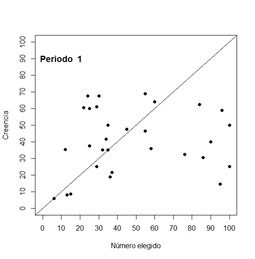
\includegraphics[width=0.45\textwidth]{Figures/F1_1} & 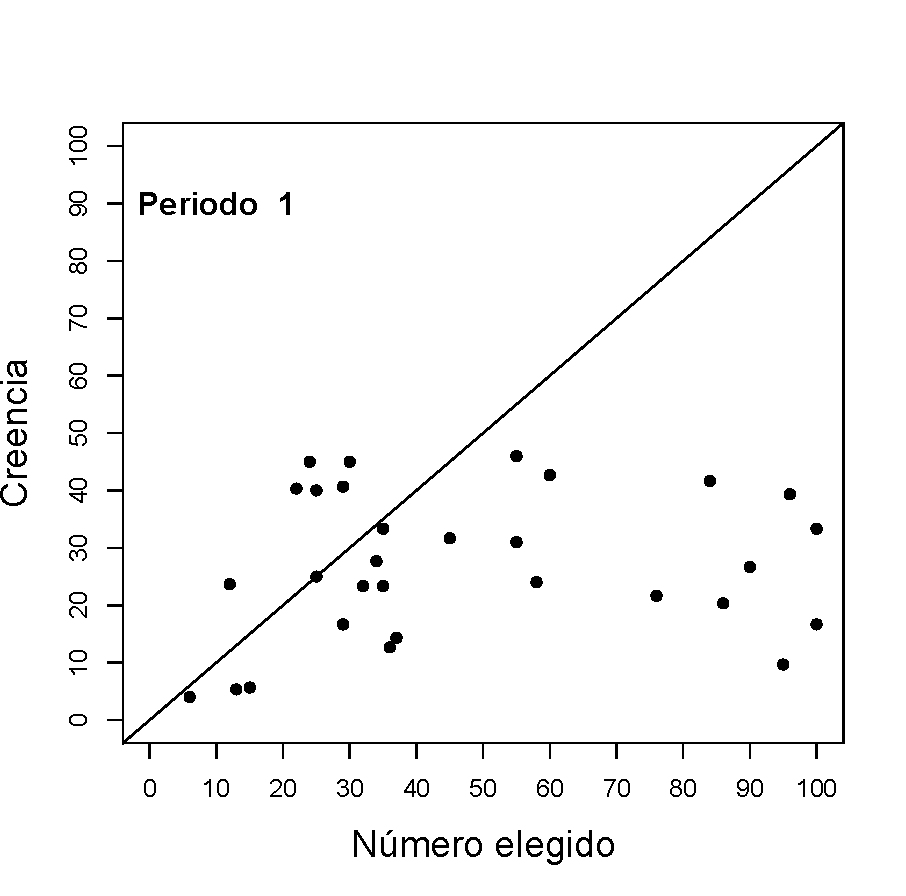
\includegraphics[width=0.45\textwidth]{Figures/F1_2} 
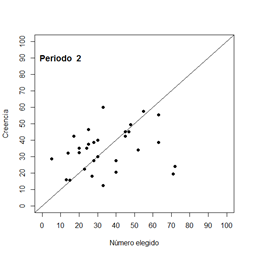
\includegraphics[width=0.45\textwidth]{Figures/F1_3} & 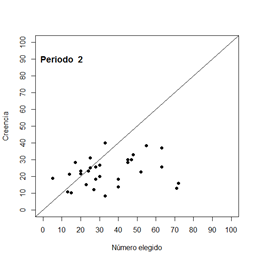
\includegraphics[width=0.45\textwidth]{Figures/F1_4} 
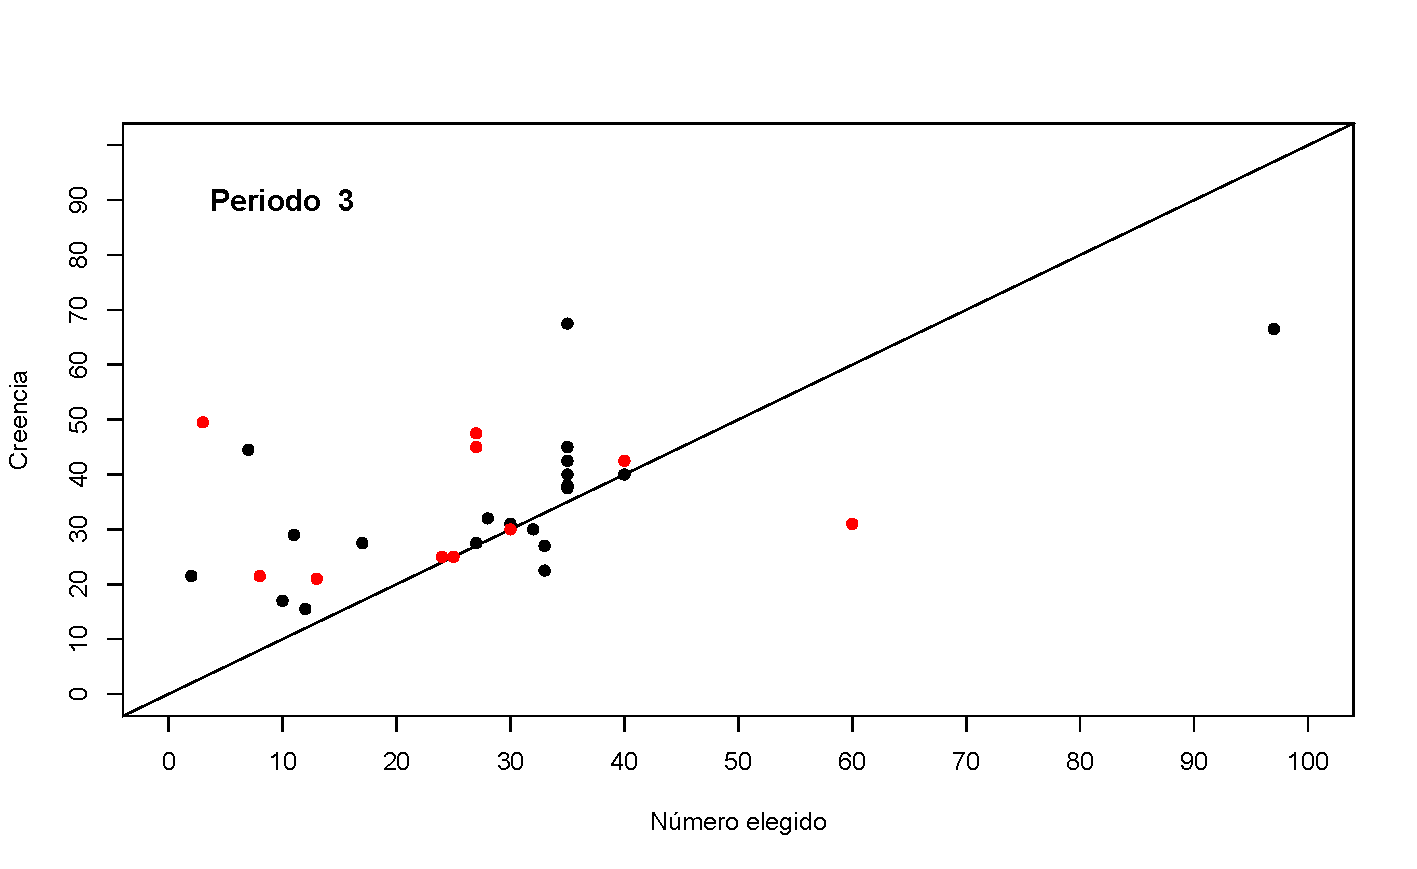
\includegraphics[width=0.45\textwidth]{Figures/F1_5} & 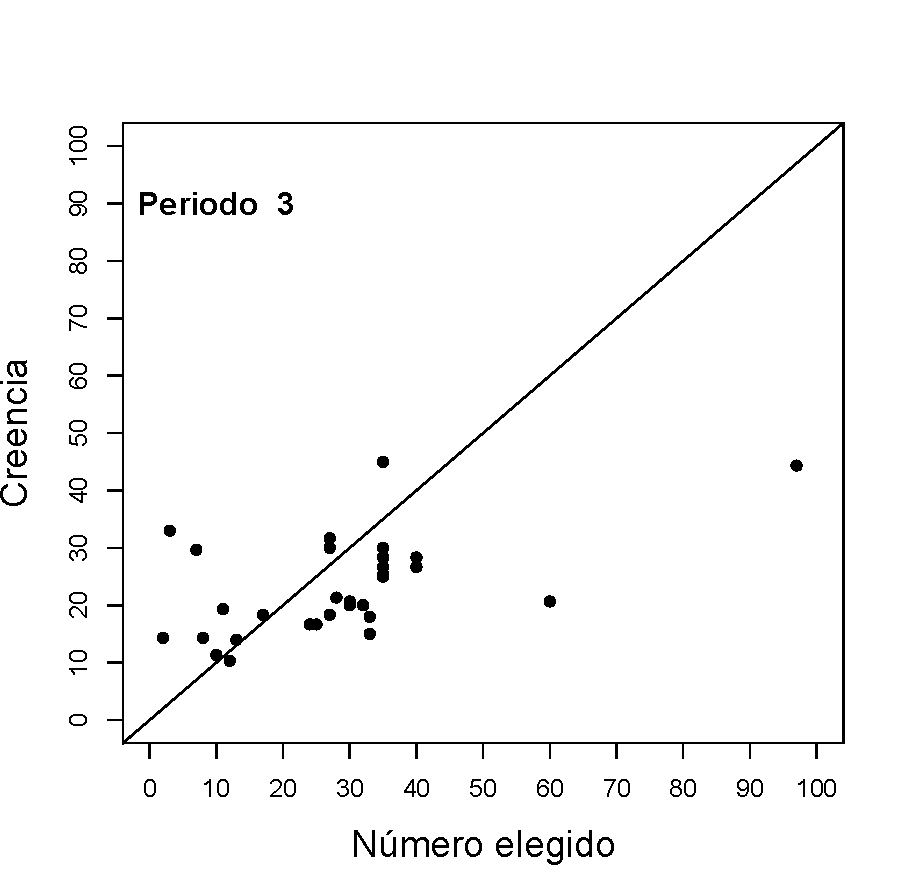
\includegraphics[width=0.45\textwidth]{Figures/F1_6} 
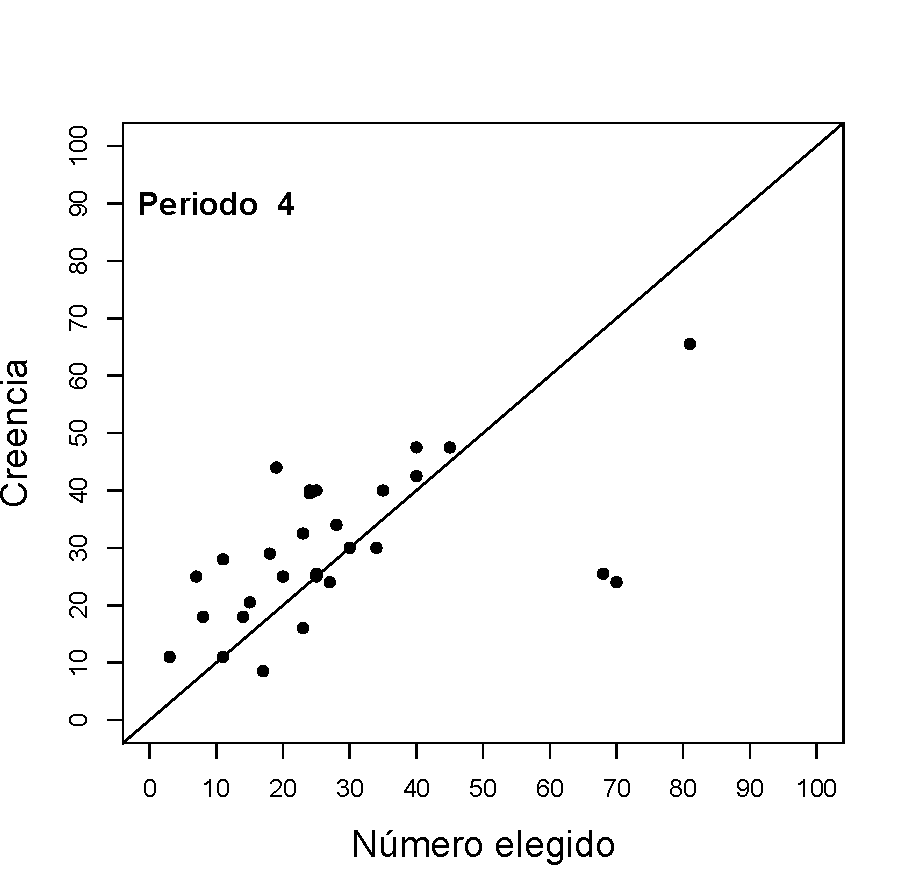
\includegraphics[width=0.45\textwidth]{Figures/F1_7} & 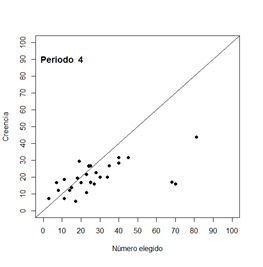
\includegraphics[width=0.45\textwidth]{Figures/F1_8} 
\decoRule
\caption[Exploración visual de la consistencia entre creencias y elecciones]{Comparación entre los números elegidos y el promedio de las creencias registradas en cada periodo. Los puntos más cercanos a la línea de identidad señalan una mayor consistencia. En las figuras del lado izquierdo las creencias promedio son multiplicadas por $p$ y en el lado derecho se omite dicha operación.}
\label{fig:Consistencia}
\end{figure}

En la Figura~\ref{fig:Consistencia} se contrasta la elección de cada participante con el promedio de las creencias registradas para cada uno de los periodos del Subjuego 1, tomando en cuenta la multiplicación por $p$ de éstas y omitiéndola (paneles izquierdos y derechos, respectivamente). Se observa que en ambos casos la diferencia entre creencias y elecciones se reduce periodo a periodo, pues en periodos posteriores los puntos se acercan más a la línea de identidad. Sin embargo, como ya se ha mencionado, esto puede deberse únicamente a que los valores elegidos se acercan más al límite inferior del espacio de elección.\\

Para evaluar la consistencia entre las creencias de los participantes y sus números elegidos tomando en cuenta el efecto de suelo, se emplearon dos métodos: el primero de ellos, computa la \textit{Diferencia Normalizada} entre las creencias y las elecciones de los participantes de acuerdo con las elecciones promedio observadas en cada periodo (Lahav, \citeyear{Lahav}); el segundo, calcula la \textit{Diferencia Relativa} entre creencias y elecciones a partir del punto medio entre ambos valores (método empleado por Slonim, \citeyear{Slonim}, para calcular el cambio relativo de los números elegidos por los jugadores de un periodo al siguiente). A su vez, tal y como lo reporta Lahav, estos métodos fueron aplicados con dos variantes para evaluar el cómputo realizado por los participantes, incluyendo u omitiendo la multiplicación del promedio de sus creencias por el parámetro $p$.\\

El procedimiento sugerido por Lahav (\citeyear{Lahav}), para calcular las diferencias normalizadas entre las creencias y las elecciones de cada participante en cada periodo, fue incorporado a partir de la siguiente ecuación:\\

\begin{center}
$DN_i^t =  \frac{(\frac{2}{3}B_i^t - C_i^t)}{\overline{C}_t} $
\end{center}

Donde $DN_i^t$ es la Diferencia Normalizada entre las creencias y elecciones de cada participante $i$ en el periodo $t$, computada a partir de la diferencia entre  la media de los números que el participante $i$ estimó que elegirían los otros dos jugadores en el periodo $t$ multiplicado por $\frac{2}{3}$, ($\frac{2}{3}B_i^t$) y el número elegido por el propio participante $i$ para ese periodo $t$ ($C_i^t$), dividida por el promedio de los números elegidos por todos los participantes en el periodo $t$ ($\overline{C}_t$).\\

Una vez computadas las diferencias por cada participante y periodo, se calculó el promedio de las mismas para poder someterlas a un análisis estadístico que permitiera evaluar si estas fueron significativamente diferentes de 0. Para ello, se realizaron pruebas t bayesianas de una sola muestra para cada periodo de juego. En la Tabla~\ref{DN-S1-B} se reportan los Factores de Bayes obtenidos en dicho análisis, que permiten estimar qué tantas veces es más probable que la evidencia corresponda con la Hipótesis Alterna (``hay diferencia entre creencias y elecciones'') respecto a la Hipótesis Nula (``no hay diferencia entre creencia y elecciones''). Como puede verse, sólamente se encontraron diferencias significativas entre creencias y elecciones en los primeros dos periodos del juego.\\

\begin{table}[h]
\caption[Diferencias Normalizadas en el Subjuego 1 (prueba t de una muestra)]{\textbf{Diferencias Normalizadas en el Subjuego 1} Prueba t bayesiana de una sola muestra que compara contra 0 el promedio de las Diferencias Normalizadas entre creencias y elecciones en el Subjuego 1.}
\label{DN-S1-B}
\centering
\begin{tabular}{l | c c | c}
\toprule
%\tabhead{Groups} & \tabhead{Treatment X} & \tabhead{Treatment Y} \\
\textbf{} & \textbf{$BF_{10}$} & \textbf{$error\%$} & \textbf{Diferencia promedio}\\
\midrule
Periodo 1 & 19.300 & 1.823e^-6 & -0.366\\
Periodo 2 & 34.545 & 3.137e^-4 & -0.342\\
Periodo 3 & 0.281 & 2.840e^-5 & -0.097\\
Periodo 4 & 0.652 & 0.015 & -0.147\\
\bottomrule
\end{tabular}
\end{table}

En la Figura~\ref{fig:DN_S1} se presenta de manera gráfica la relación entre las distribuciones prior y posterior computadas en cada periodo. Las distribuciones prior representan la Hipótesis Nula (asume diferencias  cercanas a 0) y las distribuciones posteriores presentan la magnitud de la diferencia estimada a la luz de los datos. La forma más sencilla de interpretar estas figuras es como una razón de densidades de probabilidad: si la densidad de probabilidad es mayor en la distribución prior que en la distribución posterior en el punto de "no diferencias" (que señala un tamaño del efecto 0, $\delta = 0$), quiere decir que la evidencia favorece la hipótesis alterna, ya que a la luz de la evidencia es "\textit{muy poco probable}"" (menos de lo que se esperaba de acuerdo a la distribución prior) que el tamaño de efecto tenga un valor cercano a 0.\\
  
\begin{figure}[h]
\centering
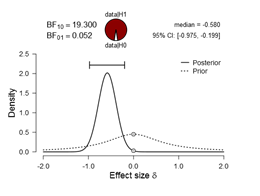
\includegraphics[width=0.45\textwidth]{Figures/F2_1} & 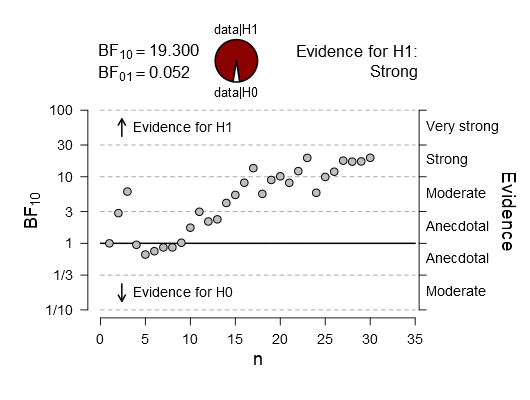
\includegraphics[width=0.45\textwidth]{Figures/F2_2} 
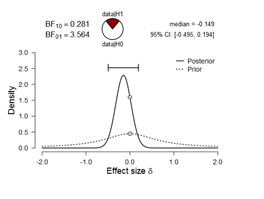
\includegraphics[width=0.45\textwidth]{Figures/F2_3} & 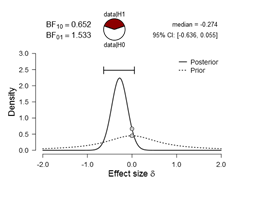
\includegraphics[width=0.45\textwidth]{Figures/F2_4} 
\decoRule
\caption[Diferencias Normalizadas entre creencias y elecciones en el Subjuegoo 1 (Factor de Bayes)]{Para la evaluación con pruebas t de una muestra de las Diferencias Normalizadas entre las creencias y las elecciones registradas el Subjuego 1, se presenta la relación entre las distribuciones prior y posteriores computadas por cada periodo. La razón de probabilidad entre estas distribuciones en el punto $\delta = 0$ señala qué tan probable es que no hayan diferencias según los datos recabados (la distribución posterior), en comparación con la hipótesis nula (la distribución prior).}
\label{fig:DN_S1}
\end{figure}

Estos resultados son consistentes con lo que reporta Lahav (\citeyear{Lahav}): en los primeros periodos no hay consistencia entre las creencias y elecciones, pero ésta parece adquirirse conforme avanzan los periodos. Así mismo, en todos los periodos se encontraron diferencias negativas, sugiriendo que en promedio las creencias de los participantes estuvieron por debajo de sus elecciones reales.\\

En el estudio presentado por Lahav (\citeyear{Lahav}), el cómputo de la Diferencia Normalizada entre las creencias y las elecciones se realizó también omitiendo la multiplicación de las creencias por $p$, en un intento por evaluar la posibilidad de que las inconsistencias halladas entre éstas y las elecciones se deban a que los participantes no habían considerado dicha operación. El presente trabajo también incorporó dicha variación del análisis, llevada a cabo de acuerdo a la siguiente ecuación, en la que se omite la multiplicación por $\frac{2}{3}$ en $B_i^t$:

\begin{center}
$DN_i^t =  \frac{(B_i^t - C_i^t)}{\overline{C}_t} $ \\
\end{center}

Nuevamente, las diferencias promedio computadas en cada periodo asumiendo que los participantes no multiplicaron sus creencias por $p$, fueron evaluadas con pruebas t bayesianas de una sola muestra.  Este análisis arrojó resultados inversos a los encontrados cuando la multiplicación por $p$ fue tomada en cuenta: los primeros periodos no muestran diferencias significativas y los últimos, sí.  Aunado a ello, las diferencias en los periodos 3 y 4 se vuelven positivas (indicando que las creencias cayeron por encima de las elecciones). Estos resultados se presentan en la Tabla~\ref{DNnop-S1-B}.\\


\begin{table}[h]
\caption[Diferencias Normalizadas en el Subjuego 1, omitiendo la multiplicación por $p$ (prueba t de una muestra)]{\textbf{Diferencias Normalizadas en el Subjuego 1 omitiendo la multiplicación por p:} Prueba t bayesiana de una sola muestra que compara contra 0 el promedio de las Diferencias Normalizadas entre las creencias (sin multiplicar por $p$) y las elecciones de los jugadores en el Subjuego 1.}
\label{DNnop-S1-B}
\centering
\begin{tabular}{l | c c | c}
\toprule
%\tabhead{Groups} & \tabhead{Treatment X} & \tabhead{Treatment Y} \\
\textbf{} & \textbf{$BF_{10}$} & \textbf{$error\%$} & \textbf{Diferencia promedio}\\
\midrule
Periodo 1 & 0.207 & 0.010 & -0.049\\
Periodo 2 & 0.196 & 0.013 & -0.012\\
Periodo 3 & 3.811 & 3.017e^-5 & 0.355\\
Periodo 4 & 1.861 & 4.032e^-4 & 0.280\\
\bottomrule
\end{tabular}
\end{table}

\begin{figure}[h]
\centering
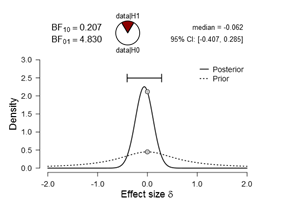
\includegraphics[width=0.45\textwidth]{Figures/F3_1} & 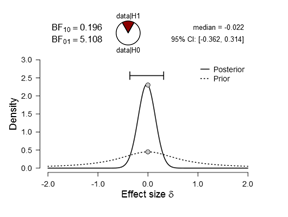
\includegraphics[width=0.45\textwidth]{Figures/F3_2} 
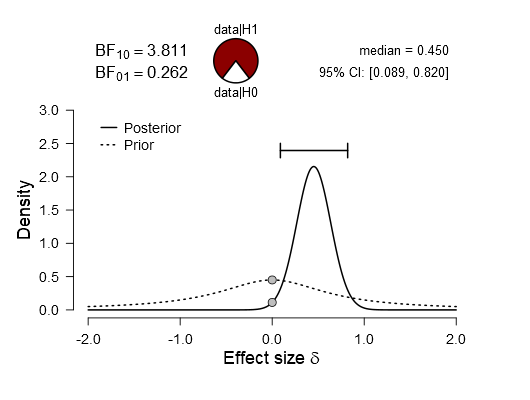
\includegraphics[width=0.45\textwidth]{Figures/F3_3} & 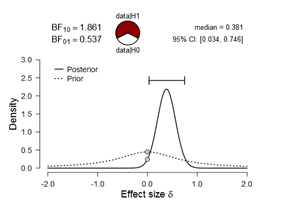
\includegraphics[width=0.45\textwidth]{Figures/F3_4} 
\decoRule
\caption[Diferencias Normalizadas entre creencias y elecciones en el Subjuegoo 1, omitiendo la multiplicación por $p$ (Factor de Bayes)]{Para la evaluación con pruebas t de una muestra de las Diferencias Normalizadas entre creencias (sin multiplicar por $p$) y elecciones en el Subjuego 1, se ilustra la relación entre las distribuciones prior y posteriores computadas por cada periodo.}
\label{fig:DNnop_S1}
\end{figure}

De acuerdo con el Factor de Bayes, aunque la Hipótesis Alterna es más probable en los periodos 3 y 4 (es decir, que sí hay diferencias entre las creencias y las elecciones) respecto de la Hipótesis Nula, la evidencia acumulada es relativamente pequeña, (particularmente en el periodo 4, donde podría considerarse anecdótica). En la Figura~\ref{fig:DNnop_S1} se muestra la relación entre las distribuciones prior y posteriores computadas por cada periodo.\\

Este resultado difiere considerablemente de los hallazgos reportados por Lahav (\citeyear{Lahav}), quien reportó que al excluir la multiplicación por $\frac{2}{3}$, las diferencias en los cuatro periodos se volvieron positivas, significativamente diferentes de 0, y en general, más grandes que cuando la multiplicación por $p$ era tomada en cuenta. En el estudio conducido por Lahav, dichos resultados fueron interpretados como un indicador de que los participantes sí toman en cuenta la multiplicación por $p$.\\

Cuando se incluye la multiplicación por $p$ en el cálculo de las Diferencias Normalizadas entre creencias y elecciones en el presente estudio, se encuentra que éstas fueron significativas en los primeros periodos, y al excluir dicha multiplicación, las diferencias significativas aparecen sólo en los últimos periodos, aunque la evidencia parece ser débil. Estos resultados podrían estar sugiriendo que los participantes comienzan el juego sin considerar la multiplicación por $\frac{2}{3}$, pero la incorporan en sus decisiones al avanzar en los periodos (o por lo menos, aprenden que el número objetivo siempre está por debajo del número promedio).\\

En general, a pesar de las diferencias en los métodos empleados para la elicitación de creencias, el presente estudio presenta hallazgos similares a los reportados por Lahav (\citeyear{Lahav}), al emplear el método propuesto para calcular las Diferencias Normalizadas entre las creencias y las elecciones de los participantes:

\begin{itemize}
\item Existen discrepancias entre las creencias y las elecciones de los participantes en los primeros periodos de juego, pero no en los últimos.\\

\item Las elecciones de los participantes suelen encontrarse entre el promedio de sus creencias respecto de los otros jugadores y el número objetivo computado de acuerdo a su multiplicación por $p$.
\end{itemize}

La diferencia más importante entre lo hallado en el presente estudio y lo reportado por Lahav (\citeyear{Lahav}), es que, en promedio, los participantes no parecen incorporar la multiplicación por $\frac{2}{3}$ en su elección, al menos en los primeros periodos.\\

Además de replicar el método de Diferencias Normalizadas utilizado por Lahav (\citeyear{Lahav}), las diferencias entre creencias y elecciones fueron evaluadas con un segundo método que no dependía de la elección promedio de todos los participantes en cada periodo para ponderarlas. La medida utilizada fue la Diferencia Relativa entre las creencias y elecciones de cada participante $i$ en cada periodo $t$, calculada de la siguiente manera:

\begin{center}
$DR_i^t =  \frac{(\frac{2}{3}B_i^t- C_i^t)}{0.5(\frac{2}{3}B_i^t + C_i^t)}$\\
\end{center}

Las Diferencias Relativas promedio computadas por cada periodo fueron evaluadas en términos de qué tanto diferían de 0, mediante la realización de pruebas t bayesianas de una sola muestra que se presentan en la Tabla~\ref{DR-S1-B}, encontrando que en tres de los cuatro periodos hubo diferencias significativas entre las creencias y elecciones. En la Figura~\ref{fig:DR_S1} se presenta la comparación entre las distribuciones prior y posterior computadas por cada periodo.\\


\begin{table}[h]
\caption[Diferencias Relativas en el Subjuego 1 (prueba t de una muestra)]{\textbf{Diferencias Relativas en el Subjuego 1} Prueba t bayesiana de una sola muestra que compara contra 0 el promedio de las Diferencias Relativas computadas entre creencias y elecciones en el Subjuego 1.}
\label{DR-S1-B}
\centering
\begin{tabular}{l | c c | c}
\toprule
%\tabhead{Groups} & \tabhead{Treatment X} & \tabhead{Treatment Y} \\
\textbf{} & \textbf{$BF_{10}$} & \textbf{$error\%$} & \textbf{Diferencia promedio}\\
\midrule
Periodo 1 & 72.283 & 7.775e^-5 & -0.457\\
Periodo 2 & 12.797 & 2.047e^-6 & -0.328\\
Periodo 3 & 0.214 & 0.008 & -0.052\\
Periodo 4 & 1.871 & 4.022e^-6 & -0.212\\
\bottomrule
\end{tabular}
\end{table}
	
\begin{figure}[h]
\centering
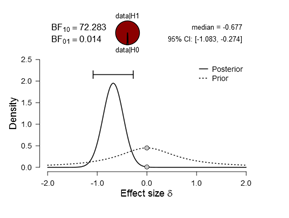
\includegraphics[width=0.43\textwidth]{Figures/F4_1} & 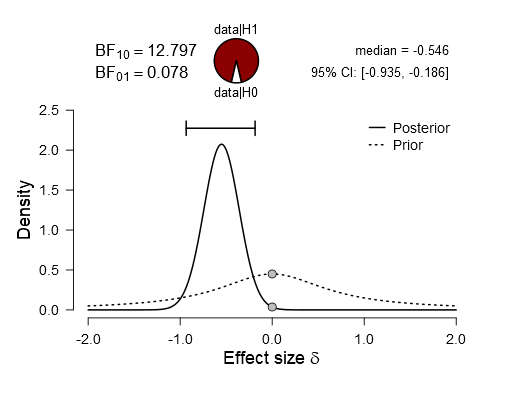
\includegraphics[width=0.43\textwidth]{Figures/F4_2} 
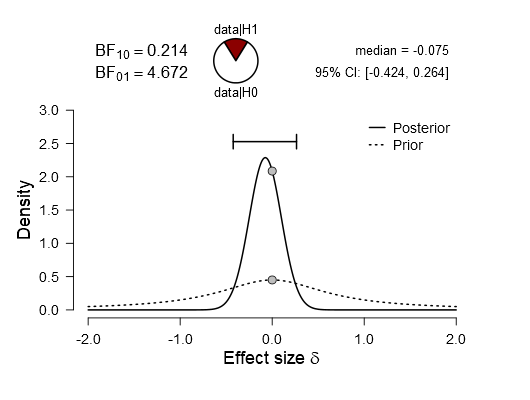
\includegraphics[width=0.43\textwidth]{Figures/F4_3} & 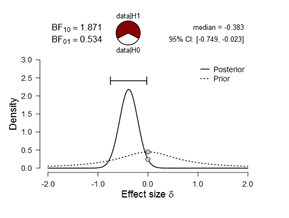
\includegraphics[width=0.43\textwidth]{Figures/F4_4} 
\decoRule
\caption[Diferencias Relativas entre creencias y elecciones en el Subjuego 1 (Factor de Bayes)]{Razón de probabilidades en el punto $\delta = 0$ entre las distribuciones prior y posterior computadas en la prueba t bayesiana con la que se evaluaron las Diferencias Relativas encontradas en el Subjuego 1.}
\label{fig:DR_S1}
\end{figure}

Tal y como se encontró con el método de Diferencias Normalizadas, todas las diferencias son negativas, indicando que consistentemente las creencias estuvieron por debajo de las elecciones reales. Sin embargo, contrario a lo que se esperaría con base en los resultados hallados con el método de Diferencias Normalizadas, donde los participantes reducen la inconsistencia entre sus elecciones y las creencias explicitadas conforme adquieren experiencia, con el método de Diferencias Relativas se observan inconsistencias (diferencias estadísticamente significativas) entre creencias y elecciones en el periodo 4, aunque no en el periodo 3. De cualquier forma, de acuerdo con el Factor de Bayes, la evidencia a favor de la hipótesis alterna en el periodo 4 es anecdótica.\\

Posteriormente, se computaron las Diferencias Relativas omitiendo la multiplicación por $p$, de acuerdo con la siguiente ecuación:

\begin{center}
$DR_i^t=  \frac{(B_i^t- C_i^t)}{0.5(B_i^t+ C_i^t)}$
\end{center}

Se realizaron pruebas t de una sola muestra para determinar si las Diferencias Relativas promedio en cada periodo son significativamente diferentes de 0, cuando la multiplicación por $p$ no es tomada en cuenta. En la Tabla~\ref{DRnop-S1-B} se presentan los resultados obtenidos y en la Figura~\ref{fig:DRnop_S1}, la relación entre las distribuciones prior y las posteriores en cada periodo.\\


\begin{table}[h]
\caption[Diferencias Relativas en el Subjuego 1, omitiendo la multiplicación por $p$ (prueba t de una muestra)]{\textbf{Diferencias Relativas en el Subjuego 1 sin la multiplicación por p} Prueba t bayesiana de una sola muestra que compara contra 0 el promedio de las Diferencias Relativas entre las creencias y las elecciones de los jugadores en el Subjuego 1, cuando las creencias no son multiplicadas por $p$.}
\label{DRnop-S1-B}
\centering
\begin{tabular}{l | c c | c}
\toprule
%\tabhead{Groups} & \tabhead{Treatment X} & \tabhead{Treatment Y} \\
\textbf{} & \textbf{$BF_{10}$} & \textbf{$error\%$} & \textbf{Diferencia promedio}\\
\midrule
Periodo 1 & 0.269 & 5.246e^-4 & -0.101\\
Periodo 2 & 0.211 & 0.009 & 0.044\\
Periodo 3 & 8.393 & 2.307e^-6 & 0.315\\
Periodo 4 & 0.810 & 5.669e^-6 & 0.167\\
\bottomrule
\end{tabular}
\end{table}
	

\begin{figure}[h]
\centering
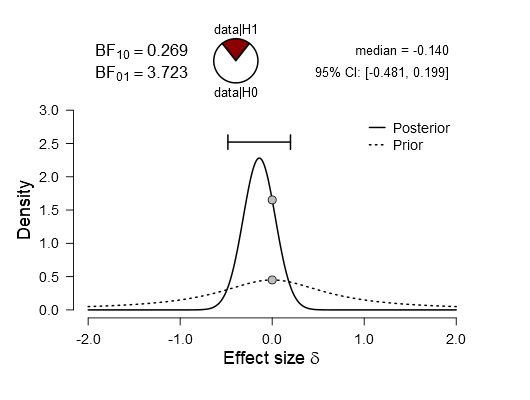
\includegraphics[width=0.45\textwidth]{Figures/F5_1} & 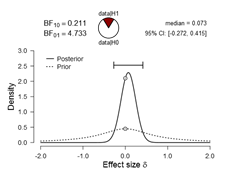
\includegraphics[width=0.45\textwidth]{Figures/F5_2} 
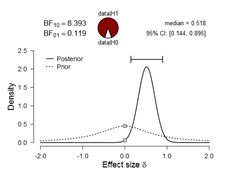
\includegraphics[width=0.45\textwidth]{Figures/F5_3} & 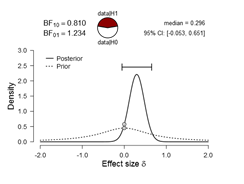
\includegraphics[width=0.45\textwidth]{Figures/F5_4} 
\decoRule
\caption[Diferencias Relativas entre creencias y elecciones en el Subjuego 1 sin la multiplicación por p (Factor de Bayes)]{Para la evaluación con pruebas t de una muestra de las Diferencias Relativas encontradas entre las creencias (sin multiplicar por $p$) y las elecciones de los participantes en el Subjuego 1, se señala la razón de probabilidades en el punto $\delta = 0$ entre las distribuciones prior y posterior.}
\label{fig:DRnop_S1}
\end{figure}


Similar a lo observado cuando se omitió la multiplicación por $p$ en el cómputo de las Diferencias Normalizadas propuesto por Lahav (\citeyear{Lahav}), se encontró una reversión en la significancia reportada en todos los periodos, (aunque nuevamente, la evidencia en el periodo 4 es anecdótica), encontrando diferencias positivas en tres de los cuatro periodos. Esto último sugiere que con el uso del método de Diferencias Relativas, en promedio, las creencias están más cercanas y ligeramente por arriba de las elecciones reales de los participantes, cuando no se toma en cuenta la multiplicación por $p$.\\

Aunque cada uno de los dos métodos empleados para evaluar la consistencia entre las creencias y elecciones de los participantes intenta compensar la tendencia hacia el equilibrio, (y el problema de suelo resultante), de forma diferente, ambos mostraron resultados muy similares: en los primeros periodos las diferencias entre creencias y elecciones son grandes, pero estas se reducen en los periodos posteriores, sugiriendo que los jugadores se vuelven consistentes conforme adquieren experiencia y aprenden también que para acercarse al número objetivo necesitan elegir números por debajo del promedio de sus creencias.

\section{Efecto de reset}\\

De acuerdo con los resultados reportados por Slonim (\citeyear{Slonim}), los jugadores presentan un efecto de ``Reset'' en la tendencia a elegir números cada vez más pequeños cuando los otros jugadores son reemplazados por jugadores nuevos, que no tienen experiencia en el juego. Tomando este hallazgo en cuenta, el presente estudio incorporó un Subjuego 2, donde sólo uno de los jugadores del Subjuego 1 permaneció jugando por otros cuatro periodos, mientras que el resto fue reemplazado por jugadores nuevos. Esta manipulación se realizó para evaluar la tendencia que en el estudio de Lahav (\citeyear{Lahav}) lleva a asumir que los jugadores se vuelven más consistentes conforme adquieren experiencia. En otras palabras, agregar un segundo Subjuego permite evaluar, con base en las respuestas del participante con experiencia, si la consistencia entre las elecciones y las creencias es algo que se adquiere con la experiencia o si es sólo el resultado del efecto de suelo asociado a la tendencia típicamente reportada en cualquier serie de juegos p-beauty contest repetido a elegir números cada vez más pequeños, (Ho, \citeyear{Teck-Hua}).\\

Para poder comparar los resultados del Subjuego 1 con el Subjuego 2, fue necesario comprobar que la incorporación de nuevos jugadores en el Subjuego 2 interrumpiera la tendencia a elegir números cada vez más pequeños en los jugadores que se mantuvieron en el juego (los participantes A). Es decir, para corroborar que el diseño experimental propuesto permite responder a la cuestión de si las diferencias entre creencias y elecciones se reducen como reflejo de una consistencia adquirida o como producto del efecto de suelo, es necesario evaluar la presencia del efecto de Reset reportado por Slonim (\citeyear{Slonim}).\\

En la Figura~\ref{fig:Reset_cambios} se muestran los cambios en las elecciones realizadas en los primeros cinco periodos consecutivos jugados por los participantes A. Los primeros tres cuadros muestran los cambios dentro del Subjuego 1 y en el cuarto panel se evalúa directamente el Efecto de Reset, al comparar la elección registrada en el último periodo del Subjuego 1 y el primer periodo del Subjuego 2. En estas gráficas, los puntos que caen por debajo de la línea de identidad indican que se eligieron números más pequeños de un periodo a otro, con lo que se observa que hay más participantes A que eligen números más pequeños entre los periodos del Subjuego 1 (por ejemplo, el $80\%$ reduce su elección entre el periodo 3 y el periodo 4), pero que esta tendencia se revierte al iniciar el subjuego 2 (el $70\%$ incrementa su número).\\

\begin{figure}[h]
\centering
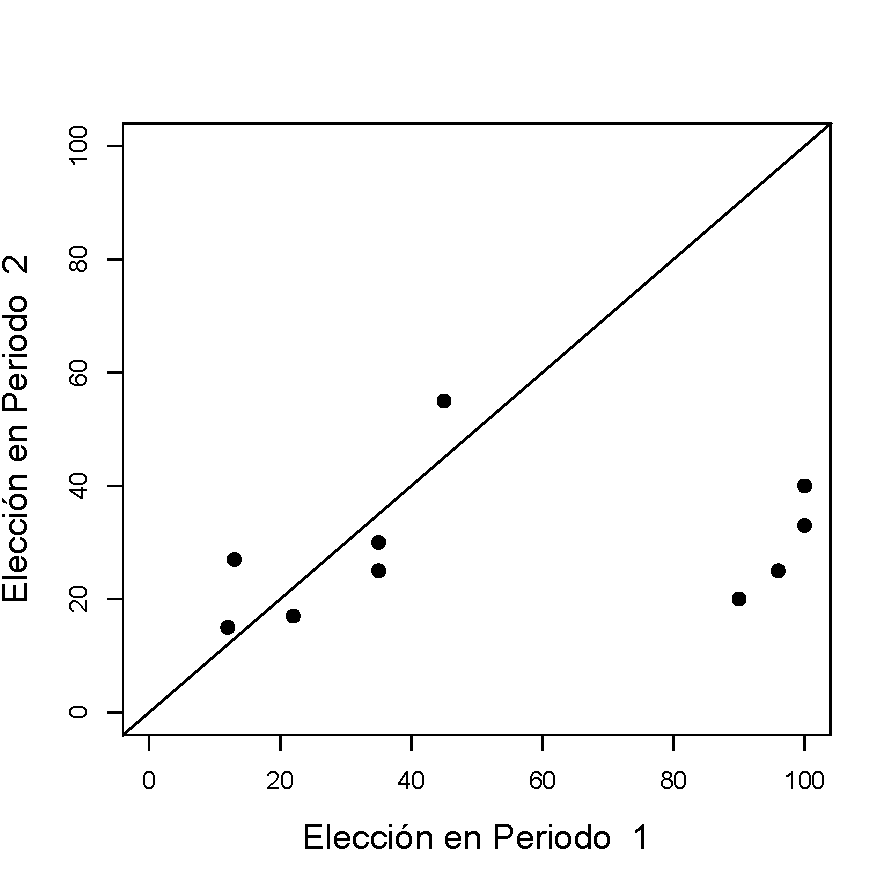
\includegraphics[width=0.45\textwidth]{Figures/F6_1} & 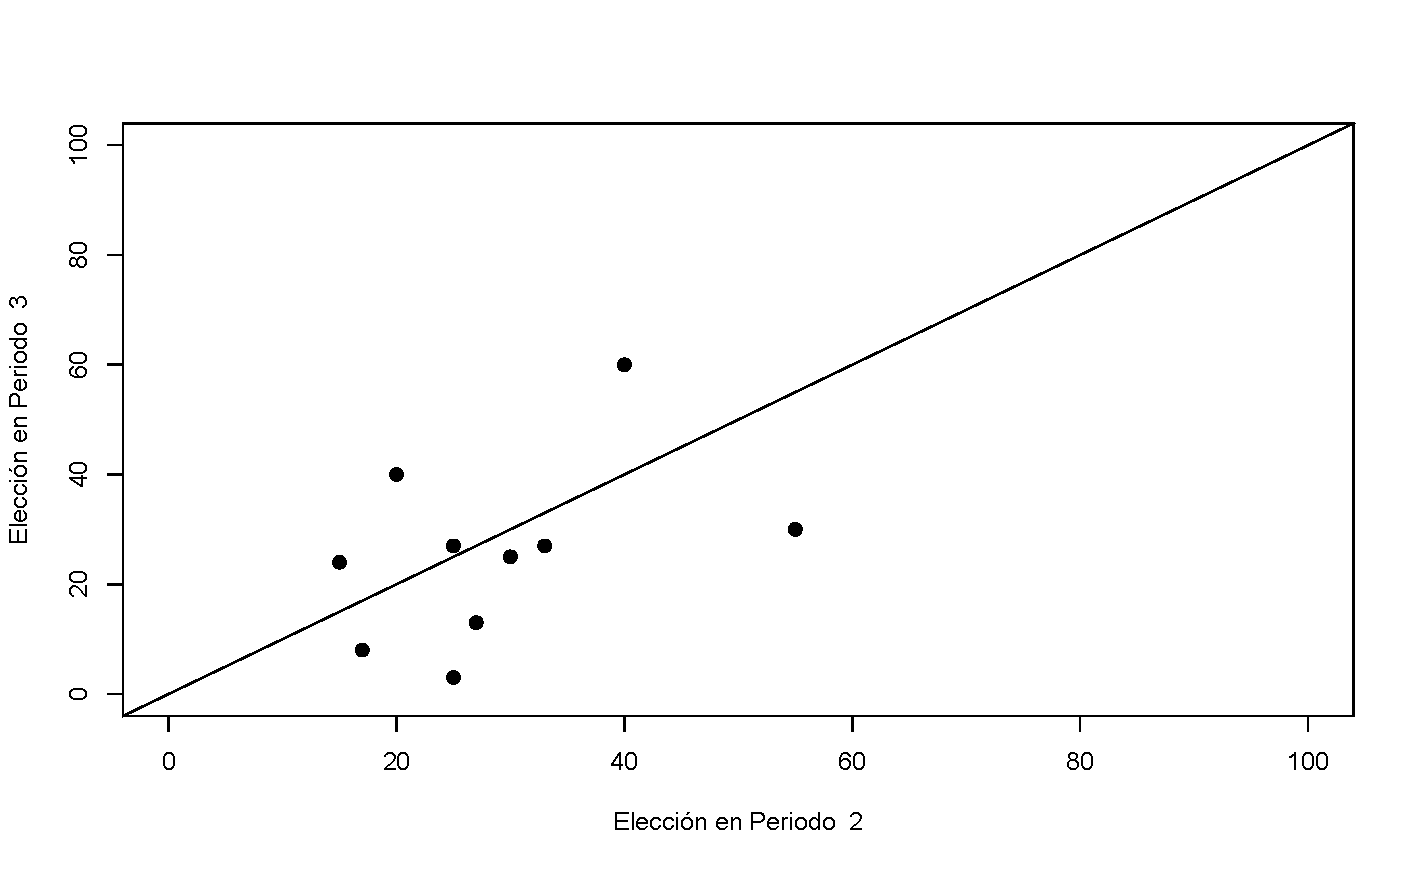
\includegraphics[width=0.45\textwidth]{Figures/F6_2} 
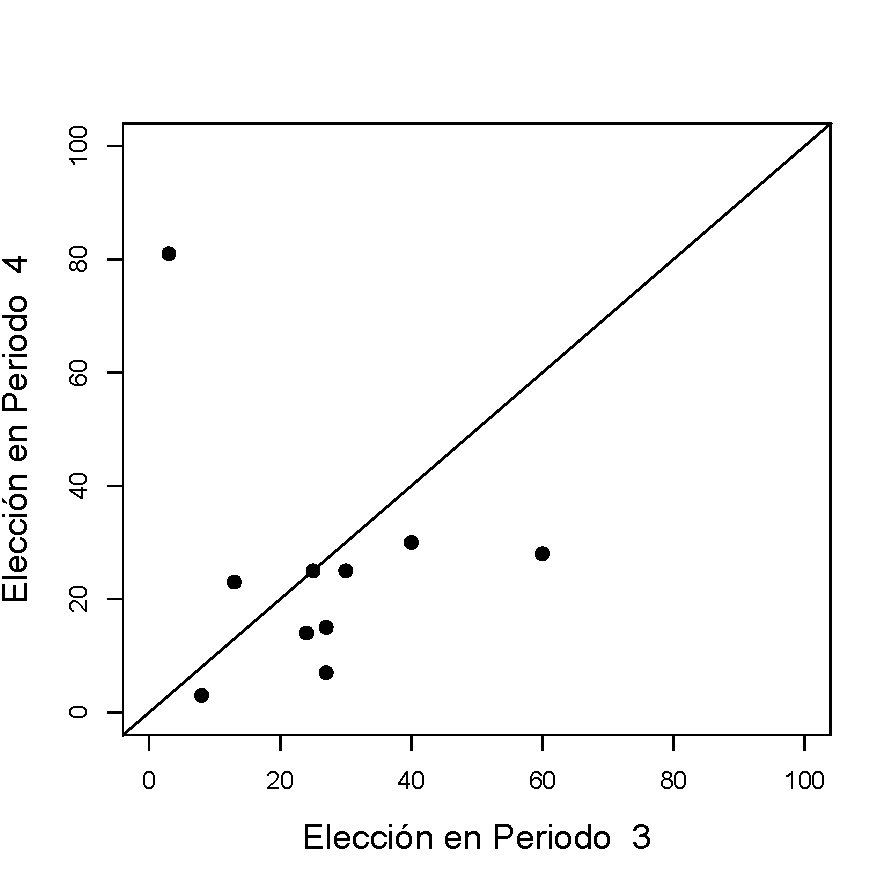
\includegraphics[width=0.45\textwidth]{Figures/F6_3} & 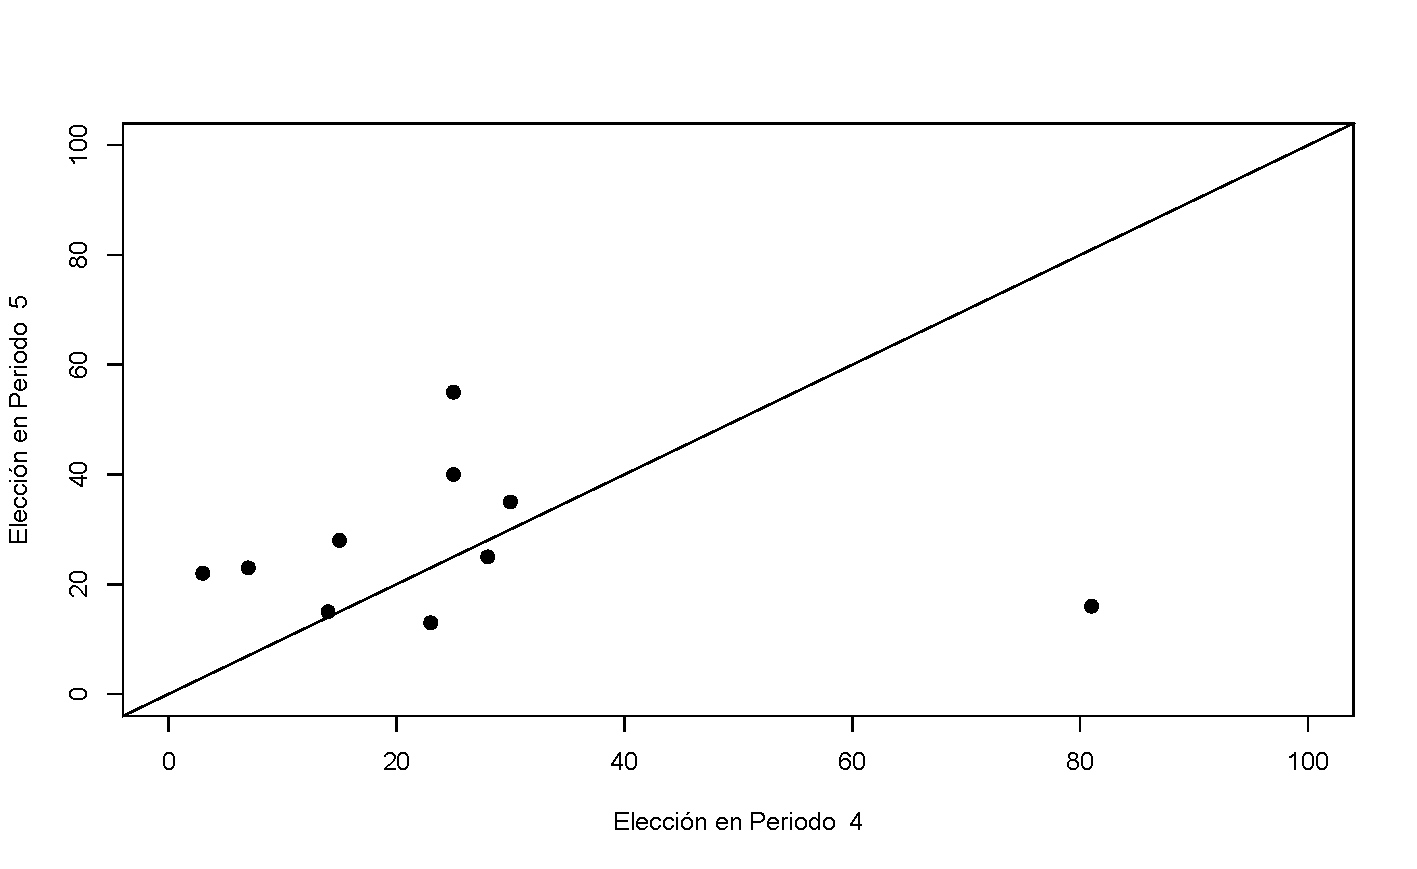
\includegraphics[width=0.45\textwidth]{Figures/F6_4} 
\decoRule
\caption[Elecciones registradas en ensayos consecutivos]{Se presenta la relación entre los números elegidos en periodos consecutivos por los participantes A, quienes jugaron los cuatro periodos del Subjuego 1 y permanecieron a lo largo del Subjuego 2. En los primeros tres páneles se aprecia que en el Subjuego 1 las elecciones tendían a disminuir, mientras que en el último panel, se observa un incremento en las mismas (el Efecto Reset).}
\label{fig:Reset_cambios}
\end{figure}

Se realizó una prueba Binomial bayesiana de una cola para comparar contra el azar la proporción de participantes A que aumentaban o disminuían sus elecciones entre cada uno de los primeros cinco periodos que jugaron (ver Tabla~\ref{Binom_Reset}), encontrando evidencia anecdótica. La falta de robustez en los resultados obtenidos en esta prueba puede deberse a que sólamente se realizaron 10 sesiones experimentales.\\

\begin{table}[h]
\caption[Prueba binomial bayesiana para evaluar la proporción de casos en que los participantes A aumentan y reducen su número elegido]{\textbf{Cambios en los números elegidos en periodos consecutivos} Prueba binomial bayesiana que compara contra el azar el número de veces que los participantes A aumentaron o disminuyeron sus números elegidos en periodos consecutivos.}
\label{Binom_Reset}
\centering
\begin{tabular}{l c | c c | c}
\toprule
%\tabhead{Groups} & \tabhead{Treatment X} & \tabhead{Treatment Y} \\
\textbf{Periodos} & \textbf{Cambio} & \textbf{Casos} & \textbf{Proporción} & \textbf{$BF_{10}$}\\
\midrule
1 vs 2 & aumentó & 3 & 0.3 & 0.176\\
       & disminuyó & 7 & 0.7 & 1.376\\
2 vs 3 & aumentó & 4 & 0.4 & 0.243\\
       & disminuyó & 6 & 0.6 & 0.643\\
3 vs 4 & aumentó & 2 & 0.2 & 0.135\\
       & disminuyó & 8 & 0.8 & 4.002\\
5 vs 6 & aumentó & 7 & 0.7 & 1.376\\
       & disminuyó & 3 & 0.3 & 0.176\\
\bottomrule
\end{tabular}
\end{table}

Para determinar si, en promedio, el número elegido por el participante A en el último periodo del Subjuego 1 es menor que el número elegido en el primer periodo del Subjuego 2, se realizó una prueba t de una cola, donde se encontró que si bien el promedio de los números elegidos en el primer periodo del Subjuego 2 es mayor que el promedio de las elecciones regitradas al final del Subjuego 1, la diferencia parece ser pequeña y no significativa.\\

No obstante, al revisar los datos de cada sesión experimental se encontraron anomalías en la ejecución del participante A de la Sesión 3, cuyo comportamiento difiere considerablemente de lo que se reporta en la literatura y en el resto de las sesiones realizadas en la presente investigación.\\

En la Figura~\ref{fig:Elecciones_ParticipantesA} se presentan las elecciones de los participantes para cada uno de los ocho periodos jugados en los dos Subjuegos, en cada una de las diez sesiones experimentales. Se puede apreciar que el participante A de la Sesión 3 no presenta la tendencia a elegir números más pequeños periodo a periodo y por el contrario, elige números muy grandes en el último periodo de cada subjuego, una estrategia que no aporta ningún tipo de ventaja en el juego. Este patrón de respuesta sugiere que el participante A de la Sesión 3 pudo no haber entendido la dinámica del juego.\\

\begin{figure}[hp]
\centering
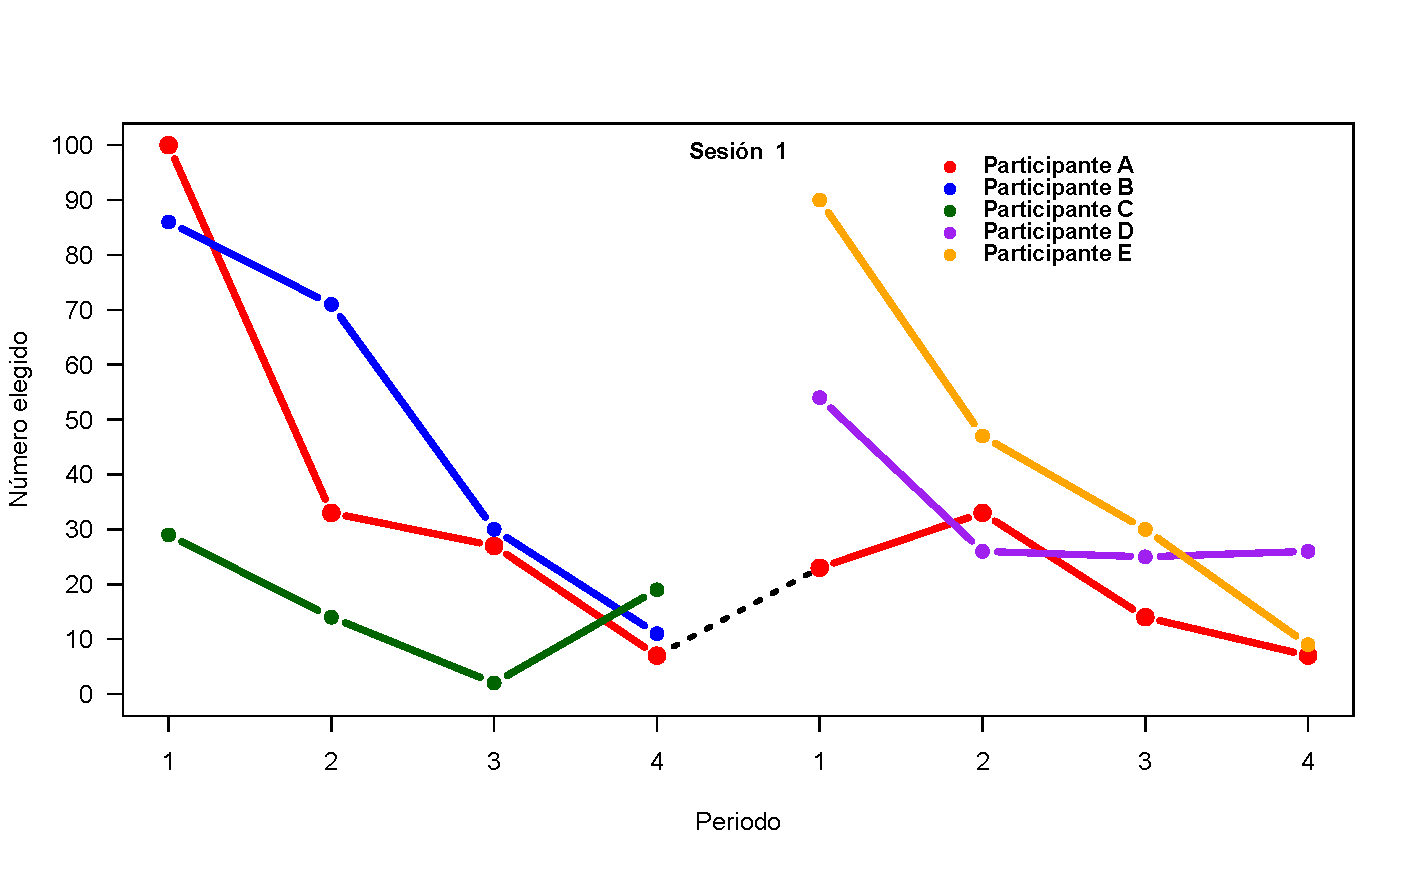
\includegraphics[width=0.45\textwidth]{Figures/F7_1} & 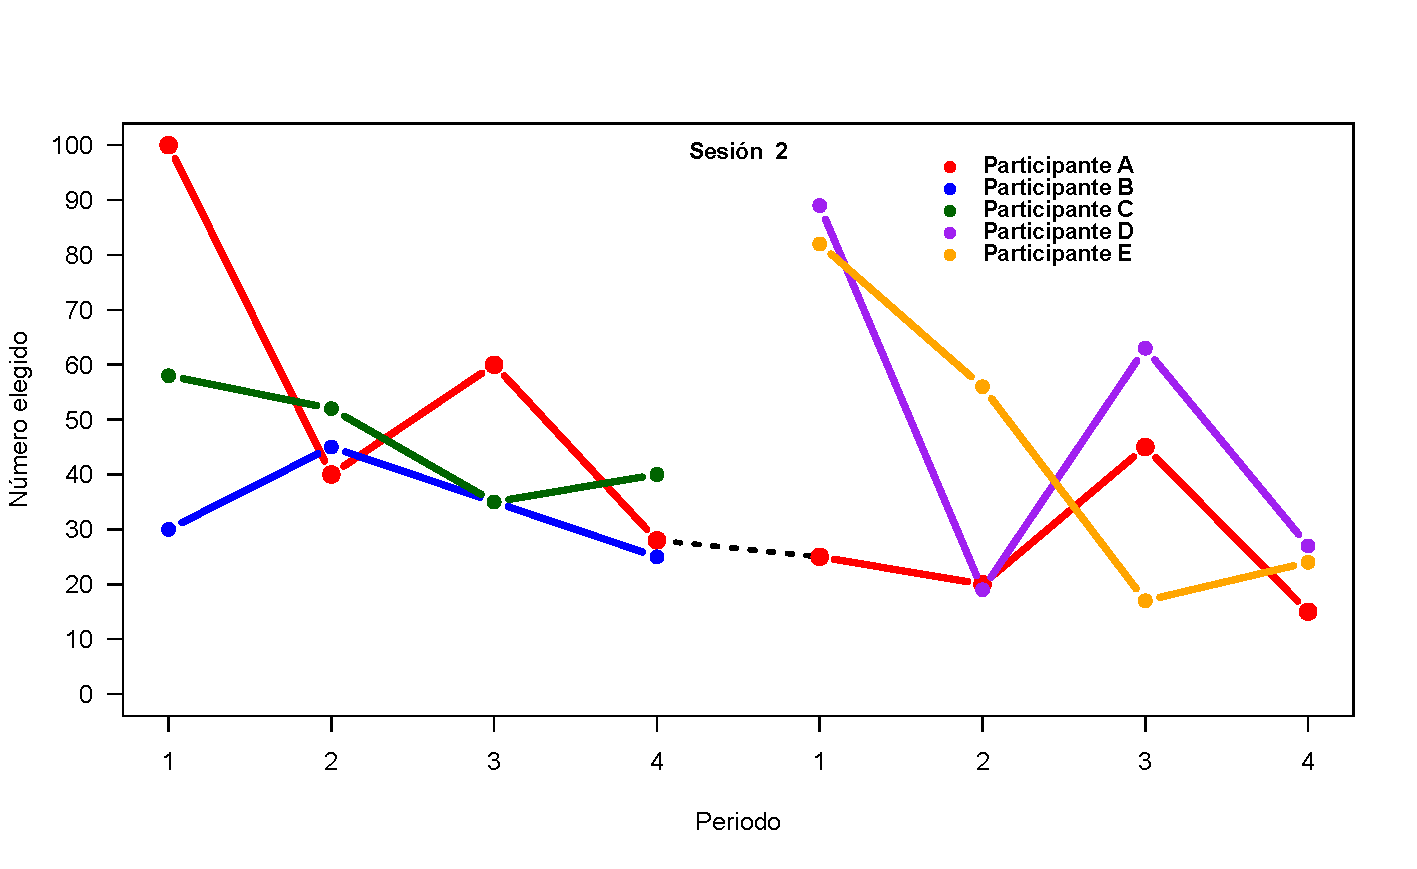
\includegraphics[width=0.45\textwidth]{Figures/F7_2} 
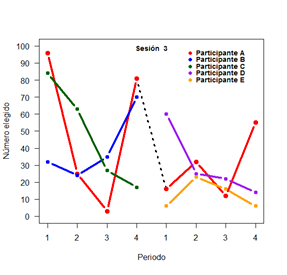
\includegraphics[width=0.45\textwidth]{Figures/F7_3} & 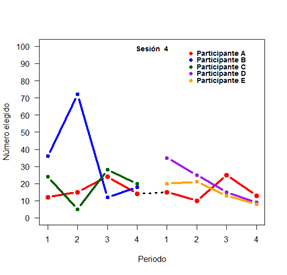
\includegraphics[width=0.45\textwidth]{Figures/F7_4} 
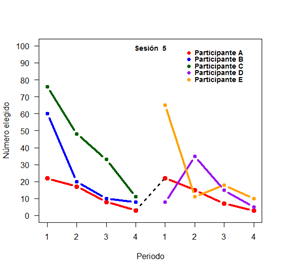
\includegraphics[width=0.45\textwidth]{Figures/F7_5} & 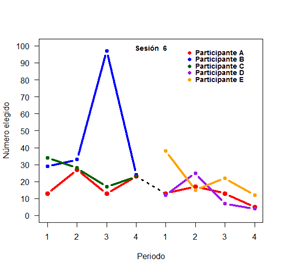
\includegraphics[width=0.45\textwidth]{Figures/F7_6} 
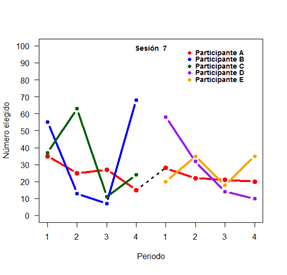
\includegraphics[width=0.45\textwidth]{Figures/F7_7} & 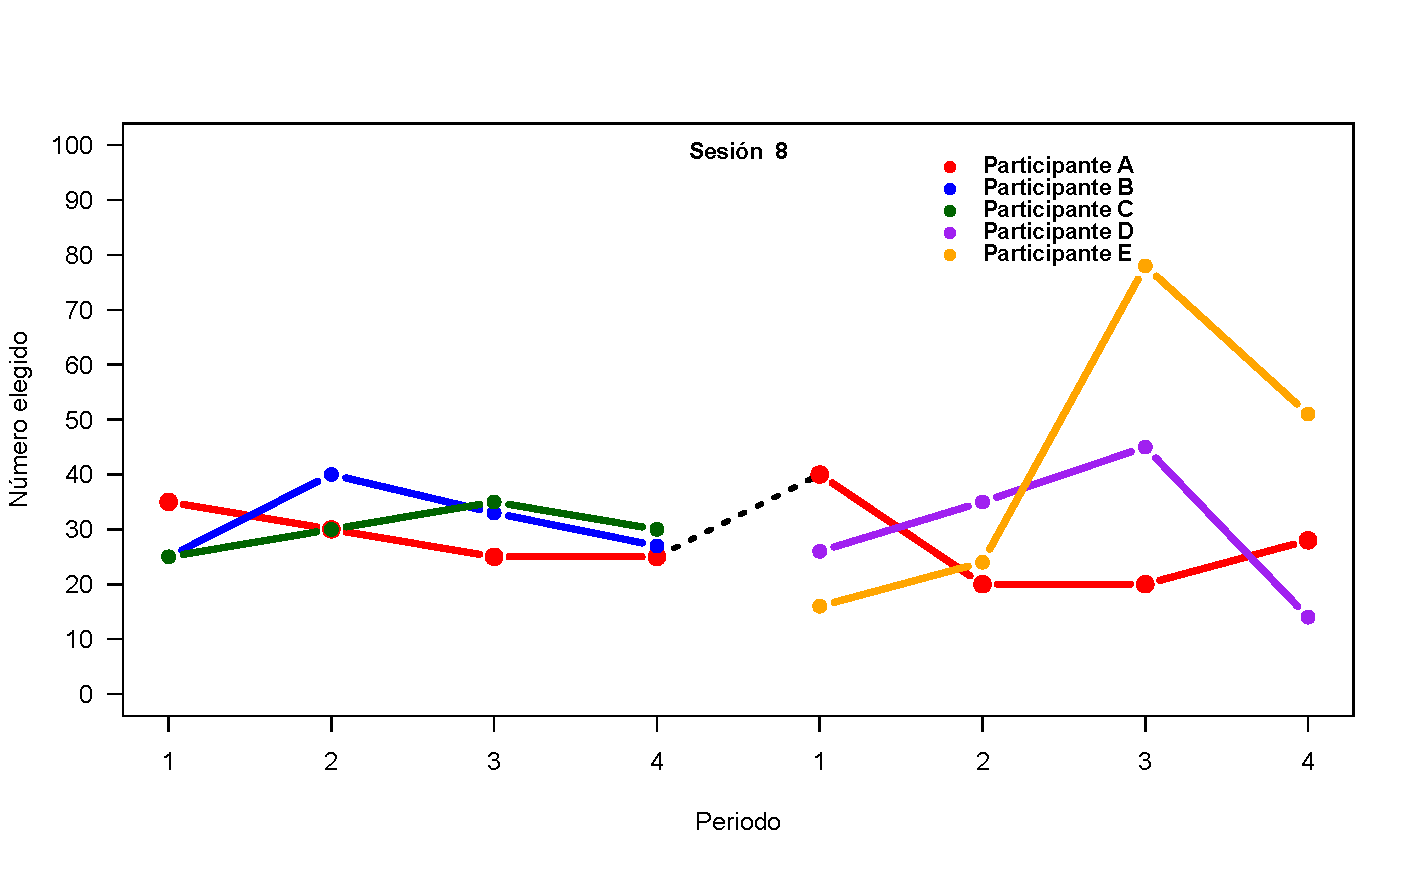
\includegraphics[width=0.45\textwidth]{Figures/F7_8} 
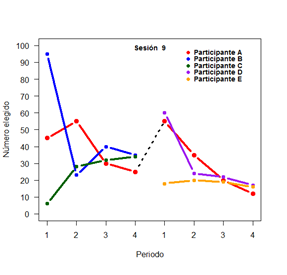
\includegraphics[width=0.45\textwidth]{Figures/F7_9} & 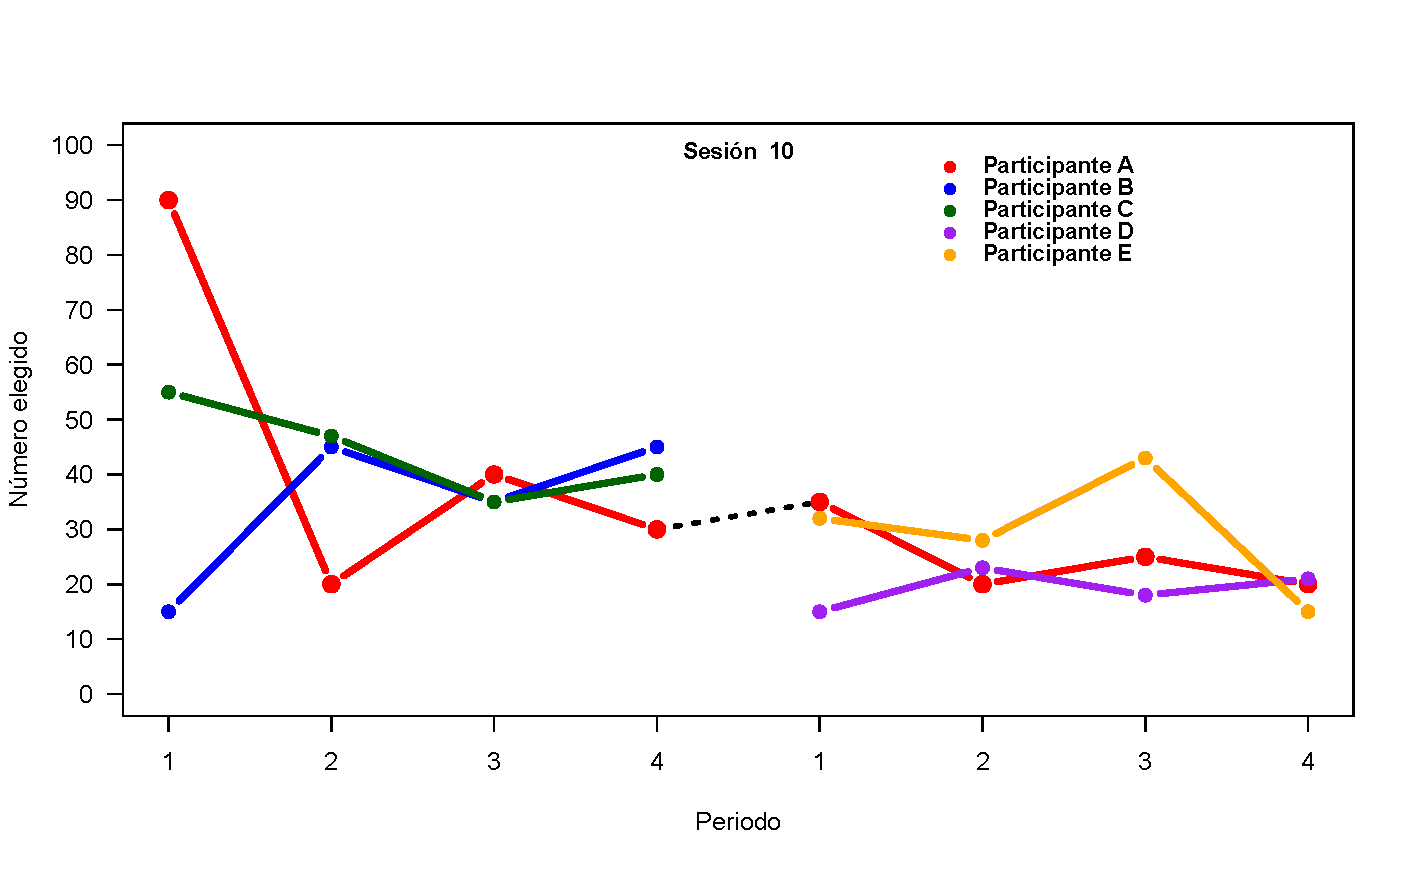
\includegraphics[width=0.45\textwidth]{Figures/F7_10} 
\decoRule
\caption[Elecciones de todos los participantes]{Se presentan todas las elecciones registradas en cada sesión experimental. Se puede apreciar que el participante A de la sesión 3 tiene un patrón atípico respecto del resto de las sesiones.}
\label{fig:Elecciones_ParticipantesA}
\end{figure}  
  
Para evaluar qué tan saliente es la tirada del participante A de la sesión 3 en el primer periodo del Subjuego 2, en la Figura~\ref{fig:Boxplot} se presentan dos diagramas: El primero, de caja y bigotes, muestra que la elección realizada por el jugador A de la Sesión 3 en el primer periodo se encuentra por arriba del rango intercuadrático multiplicado por 1.5, lo que permite clasificarla como un valor atípico.  El  segundo diagrama, de violín, complementa la información del diagrama de caja y bigotes con un diagrama de densidad a los lados; la forma externa del diagrama representa todos los resultados posibles, y el grosor indica qué tan comúnes son.\\

\begin{figure}[hp]
\centering
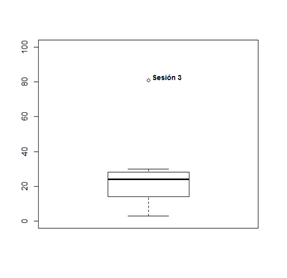
\includegraphics[width=0.45\textwidth]{Figures/F8_1} & 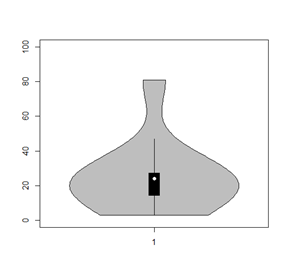
\includegraphics[width=0.45\textwidth]{Figures/F8_2} 
\decoRule
\caption[Participante atípico: Comparando el desempeño del Participante A de la Sesión 3]{Contraste entre el Participante A de la Sesión 3 y el resto de los Participantes A. Del lado izquiero se presenta un diagrama de caja y bigotes y del lado derecho, un diagrama de violín que complementa esta información con un diagrama de densidad.}
\label{fig:Boxplot}
\end{figure}  

Tomando en cuenta dicho resultado, se repitieron las pruebas t de una cola para comprobar que el número elegido por los participantes A en el último periodo del Subjuego 1 son más pequeños que el número elegido en el primer periodo del Subjuego 2, omitiendo al participante A de la Sesión 3. Al realizar dicho análisis, el número elegido en promedio por los participantes A en el último periodo del Subjuego 1 fue significativamente menor que la elección promedio registrada en el primer periodo del Subjuego 2, encontrando evidencia del efecto de Reset (prueba clásica $t = -2.317$, $p = .025 < 0.5$, prueba bayesiana $BF_{10} = 3.57$, $error = 1.377e-4$).\\

En la Figura~\ref{fig:ParticipantesA_promedio} se presenta el promedio de los números elegidos por los participantes A y los participantes no-A (participantes B y C, D y E para los Subjuegos 1 y 2, respectivamente) en cada periodo. Se presentan en gráficos diferentes los promedios computados cuando se consideran los datos de la Sesión 3 (panel izquierdo) y cuando no (panel derecho).\\
  
\begin{figure}[h]
\centering
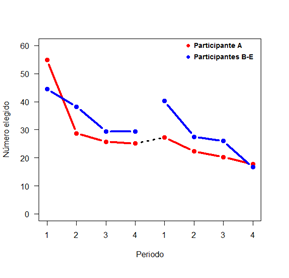
\includegraphics[width=0.45\textwidth]{Figures/F9_1} & 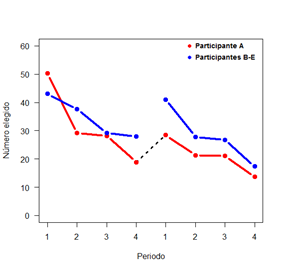
\includegraphics[width=0.45\textwidth]{Figures/F9_2} 
\decoRule
\caption[Promedio de los números elegidos por los participantes A y no-A en cada uno de los periodos jugados]{Se presenta el promedio de los números elegidos en cada uno de los periodos jugados por los participantes A (en color rojo) y los participantes B y C en el Subjuego 1, y D y E en el Subjuego 2 (en color azul). La gráfica de la izquierda incorpora los datos obtenidos en la Sesión 3 y la gráfica de la derecha, no.}
\label{fig:ParticipantesA_promedio}
\end{figure}  

Con base en estos resultados, se puede afirmar que se logró replicar el efecto de Reset reportado por Slonim (\citeyear{Slonim}), omitiendo los datos recopilados de la Sesión 3. Con ello, se comprueba la validez en la comparación de la consistencia entre las creencias y elecciones de los participantes A en cada periodo, a lo largo de los dos subjuegos.

\section{Consistencia entre creencias y elecciones entre subjuegos}\\

Las creencias y elecciones de los participantes en el Subjuego 2 fueron sometidos a los mismos análisis reportados para el Subjuego 1 en la \textbf{sección 4.2}: se computaron las Diferencias Normalizadas y las Diferencias Relativas, incluyendo y excluyendo la multiplicación por $p$. Pero en esta ocasión, se hizo una distinción entre la ejecución de los jugadores con experiencia (participantes A) y los jugadores que participaban en el juego por primera vez (participantes D y E).\\

\begin{figure}[ph]
\centering
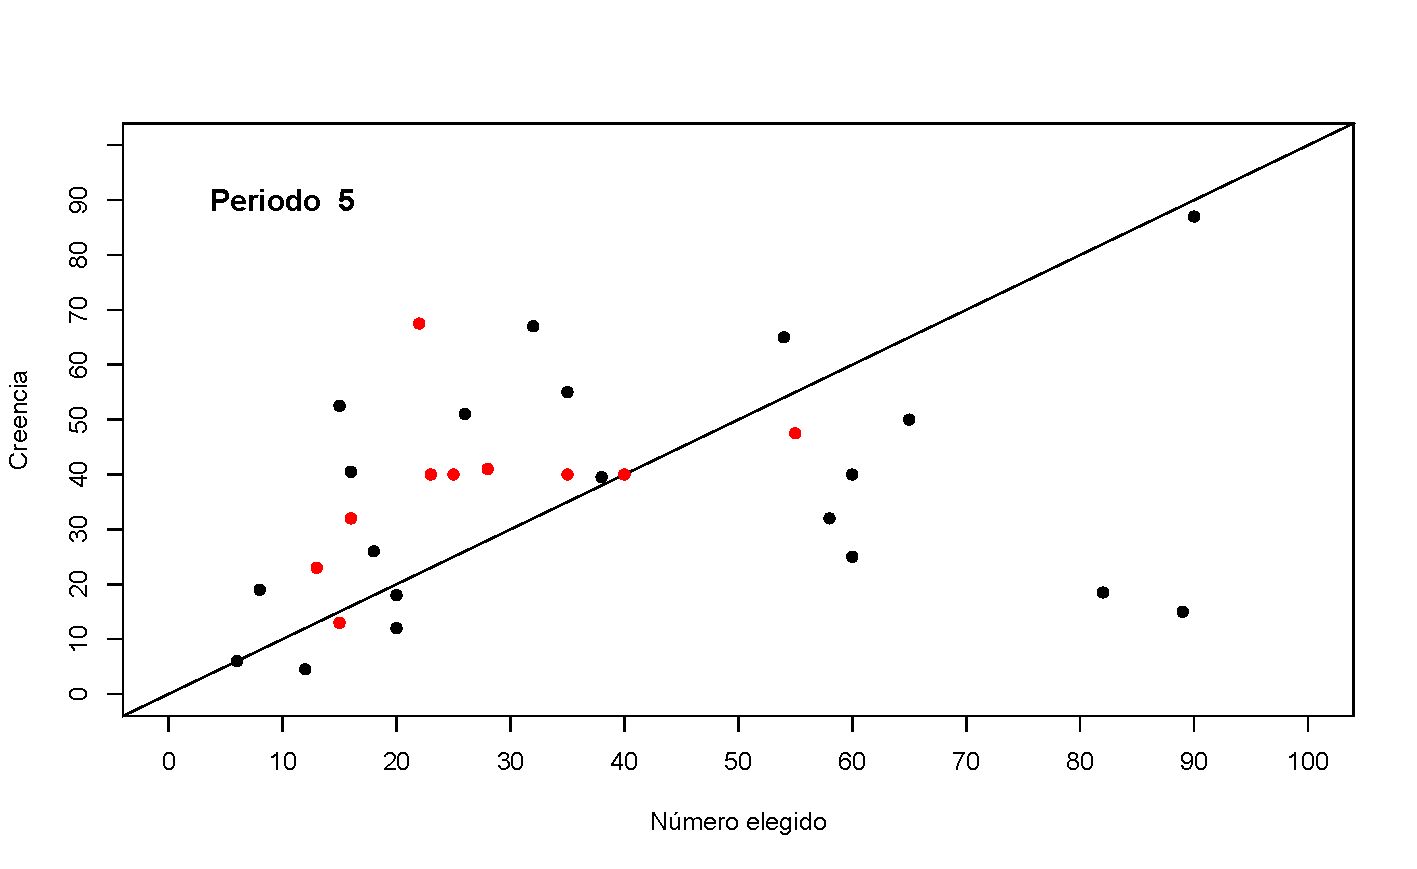
\includegraphics[width=0.45\textwidth]{Figures/F10_1} & 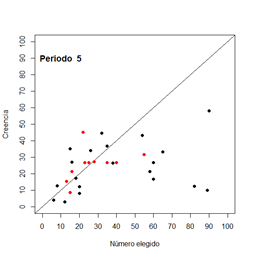
\includegraphics[width=0.45\textwidth]{Figures/F10_2} 
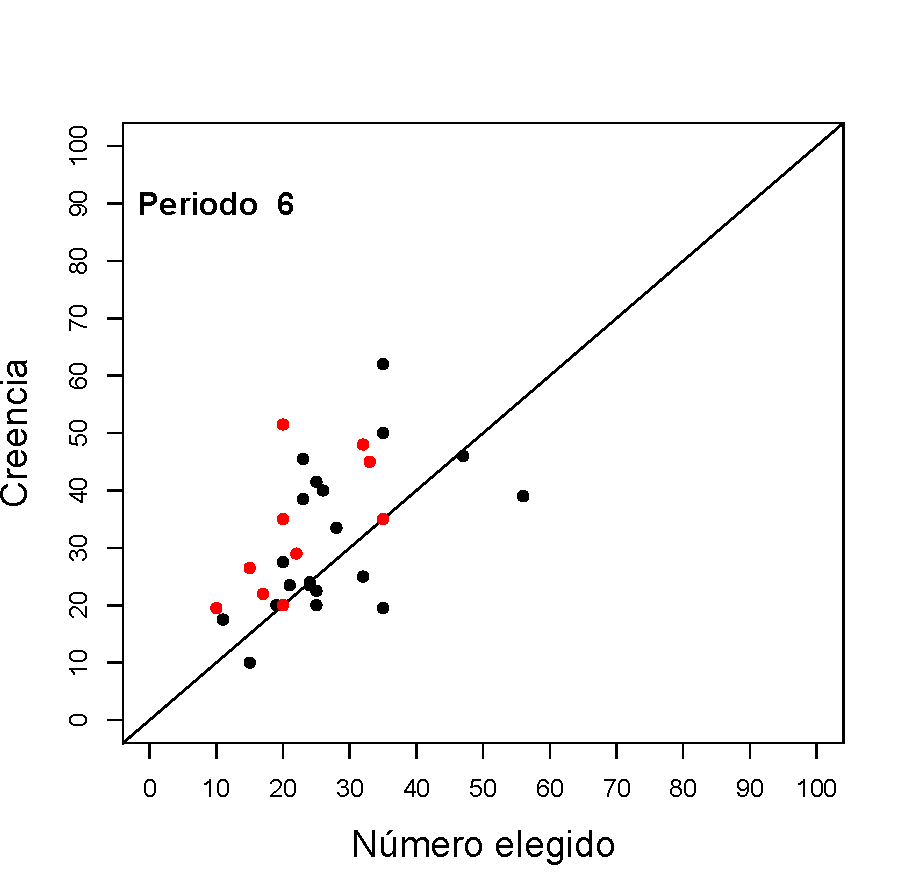
\includegraphics[width=0.45\textwidth]{Figures/F10_3} & 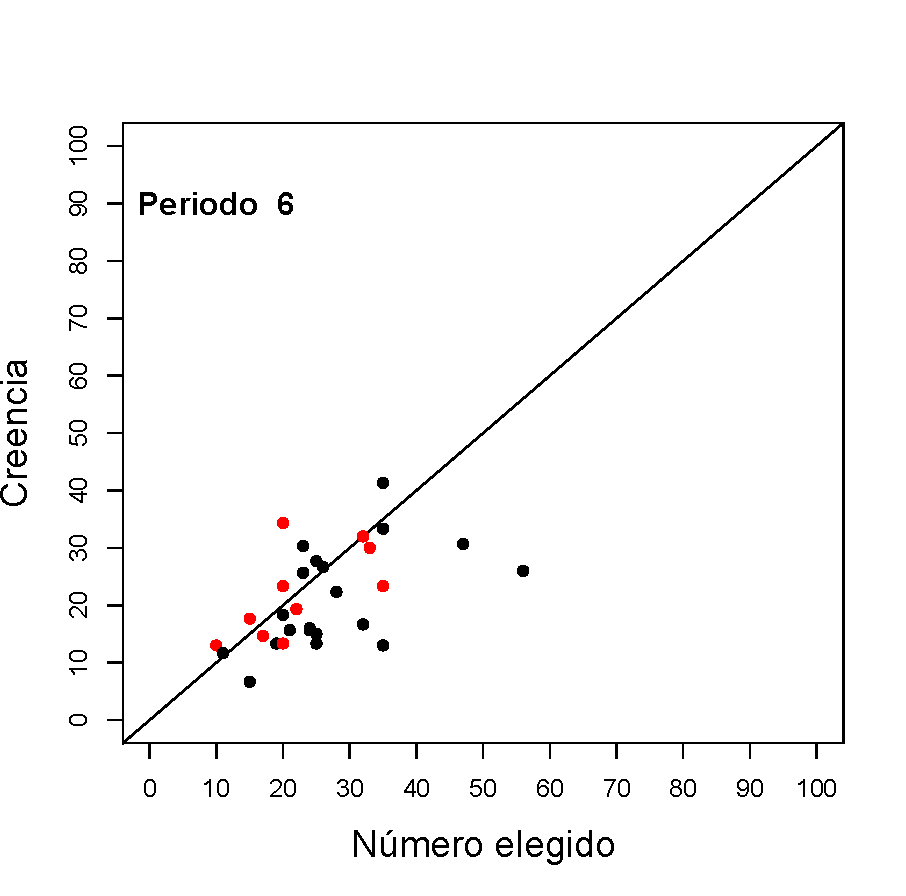
\includegraphics[width=0.45\textwidth]{Figures/F10_4} 
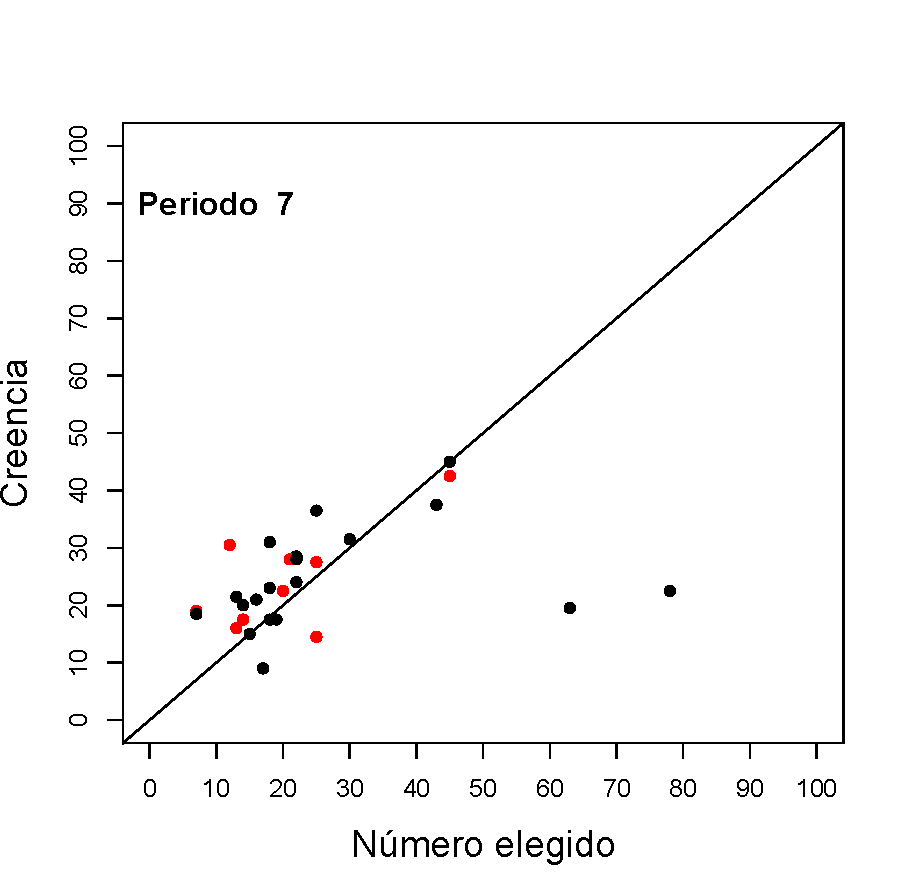
\includegraphics[width=0.45\textwidth]{Figures/F10_5} & 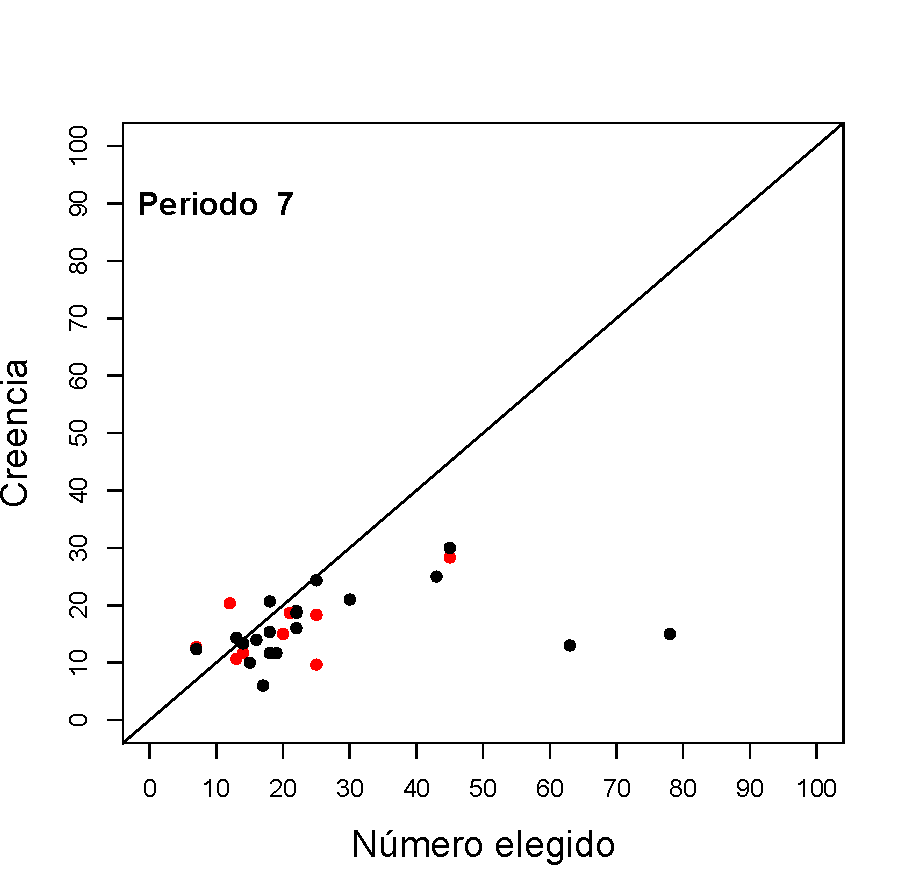
\includegraphics[width=0.45\textwidth]{Figures/F10_6} 
\includegraphics[width=0.45\textwidth]{Figures/F10_7} & \includegraphics[width=0.45\textwidth]{Figures/F10_8} 
\decoRule
\caption[Comparación enter las creencias y elecciones registradas en el Subjuego 2]{Se presenta la relación entre el promedio de las creencias registradas en cada periodo por los participantes del Subjuego 2 y sus elecciones, cuando sus creencias son multiplicadas por $p$ (paneles izquierdos) o no (páneles derechos). Los participantes A, con la experiencia del Subjuego 1, se señalan en rojo.}
\label{fig:Consistencia_promedio}
\end{figure}  

En la Figura~\ref{fig:Consistencia_promedio} se contrasta la elección de cada participante con su creencia promedio en cada uno de los periodos del subjuego 2, cuando se incluye la multiplicación por $p$ y cuando esta se omite. Los participantes A están marcados en rojo. En general, se observa que estos participantes fueron más consistentes en sus creencias y elecciones comparados con los participantes D y E.\\

Se calculó la Diferencia Normalizada entre las creencias y elecciones registradas en cada periodo del Subjuego 2, por los participantes A y los participantes D y E. Posteriormente,  se realizaron pruebas t bayesianas para determinar si estas diferencias fueron estadísticamente diferentes de 0.

\begin{table}[h]
\caption[Diferencias Normalizadas en el Subjuego 2; Participante A (Pruebas t de una muestra)]{\textbf{Diferencias Normalizadas en el Subjuego 2 (Participantes A)} Se presentan los resultados de una prueba t de una muestra que compara contra 0 las Diferencias Normalizadas computadas para los participantes A en el Subjuego 2}
\label{DN-S2-A-B}
\centering
\begin{tabular}{l | c c | c}
\toprule
%\tabhead{Groups} & \tabhead{Treatment X} & \tabhead{Treatment Y} \\
\textbf{} & \textbf{$BF_{01}$} & \textbf{$error\%$} & \textbf{Diferencia promedio}\\
\midrule
Periodo 5 & 3.010 & 0.006 & -0.049\\
Periodo 6 & 3.212 & 0.007 & -0.011\\
Periodo 7 & 2.012 & 0.003 & -0.133\\
Periodo 8 & 3.205 & 0.007 & -0.028\\
\bottomrule
\end{tabular}
\end{table}

\begin{table}[h]
\caption[Diferencias Normalizadas en el Subjuego 2; Participantes D y E (Pruebas t de una muestra)]{\textbf{Diferencias Normalizadas en el Subjuego 2 (Participantes D y E)} Se presentan los resultados de una prueba t de una muestra que compara contra 0 las Diferencias Normalizadas computadas para los participantes D y E en el Subjuego 2}
\label{DN-S2-DyE-B}
\centering
\begin{tabular}{l | c c | c}
\toprule
%\tabhead{Groups} & \tabhead{Treatment X} & \tabhead{Treatment Y} \\
\textbf{} & \textbf{$BF_{01}$} & \textbf{$error\%$} & \textbf{Diferencia promedio}\\
\midrule
Periodo 5 & 0.315 & 0.003 & -0.349\\
Periodo 6 & 0.102 & 6.001e-4 & -0.243\\
Periodo 7 & 0.063 & 2.519e^-4 & -0.307\\
Periodo 8 & 4.002 & 0.022 & -0.047\\
\bottomrule
\end{tabular}
\end{table}
  

En las Tablas~\ref{DN-S2-A-B} y \ref{DN-S2-DyE-B} se presentan los resultados obtenidos en las pruebas t bayesianas de una sola muestra que evalúan el promedio de las Diferencias Normalizadas computadas entre creencias y elecciones contra 0. De acuerdo con la Tabla~\ref{DN-S2-A-B}, los participantes A no mostraron diferencias significativas (el factor de Bayes en este caso indica qué tantas veces es más probable que no haya diferencias), lo que indica una mayor consistencia entre sus creencias y elecciones en todos los periodos del Subjuego 2. En contraste, en la Tabla~\ref{DN-S2-DyE-B} se puede observar que los participantes D y E mostraron diferencias significativas en los primeros tres periodos del subjuego, y sólo parecieron  adquirir consistencia entre sus creencias y elecciones en el último periodo. Este último resultado es muy similar a lo reportado en los participantes del Subjuego 1, donde todos los jugadores compartían el mismo nivel de experiencia. Además, en todos los casos, las creencias estuvieron por debajo de las elecciones reales. En las Figuras~\ref{fig:DN_S2_A} y \ref{fig:DN_S2_DyE} se incluyen las distribuciones prior y posterior de las Diferencias Normalizadas por periodo para los participantes A y los participantes D y E, respectivamente.\\ 

\begin{figure}[h]
\centering
\includegraphics[width=0.45\textwidth]{Figures/F11_1} & \includegraphics[width=0.45\textwidth]{Figures/F11_2} 
\includegraphics[width=0.45\textwidth]{Figures/F11_3} & \includegraphics[width=0.45\textwidth]{Figures/F11_4} 
\decoRule
\caption[Evaluación de las Diferencias Normalizadas entre creencias y elecciones en los participantes A en el Subjuego 2 (Factor de Bayes)]{Como resultado de la evaluación de las Diferencias Normalizadas computadas para los participantes A en el Subjuego 2, se presenta la comparación entre las distribuciones prior y posterior computadas por cada periodo, en el punto de no diferencias ($\delta = 0$).}
\label{fig:DN_S2_A}
\end{figure}  


\begin{figure}[h]
\centering
\includegraphics[width=0.45\textwidth]{Figures/F12_1} & \includegraphics[width=0.45\textwidth]{Figures/F12_2} 
\includegraphics[width=0.45\textwidth]{Figures/F12_3} & \includegraphics[width=0.45\textwidth]{Figures/F12_4} 
\decoRule
\caption[Evaluación de las Diferencias Normalizadas entre creencias y elecciones en los participantes D y E en el Subjuego 2 (Factor de Bayes)]{Como resultado de la evaluación de las Diferencias Normalizadas computadas para los participantes D y E en el Subjuego 2, se presenta la comparación entre las densidades de probabilidad de las distribuciones prior y posterior computadas por periodo, en el punto de no diferencias.}
\label{fig:DN_S2_DyE}
\end{figure}  

Se repitió el cálculo de las Diferencias Normalizadas en los cuatro periodos del Subjuego 2 omitiendo la multiplicación por $p$, con el propósito de evaluar si los jugadores tomaron en cuenta este cálculo en la elección de su número. Tras la realización de las pruebas t bayesianas de una sola muestra correspondientes,  sólo se encontraron diferencias significativas entre las elecciones y las creencias de los participantes A en los dos primeros  periodos, (ver Tabla~\ref{DNnop-S2-A-B}). En general, la magnitud de las diferencias parece ser mayor en todos los periodos cuando se excluye la multiplicación por $p$ que cuando esta sí se incluye. Este resultado sugiere que los jugadores con experiencia previa sí tomaron en cuenta la multiplicación por $p$, o por lo menos, que aprendieron desde el Subjuego 1 que el número objetivo siempre está por debajo del promedio de los números elegidos.\\

\begin{table}[h]
\caption[Diferencias Normalizadas en el Subjuego 2 omitiendo la multiplicación por $p$; Participante A (Pruebas t de una muestra)]{\textbf{Diferencias Normalizadas en el Subjuego 2 (Participantes A)} Se presentan los resultados de una prueba t de una muestra que compara contra 0 las Diferencias Normalizadas computadas para los participantes A en el Subjuego 2, cuando las creencias registradas no son multiplicadas por $p$.}
\label{DNnop-S2-A-B}
\centering
\begin{tabular}{l | c c | c}
\toprule
%\tabhead{Groups} & \tabhead{Treatment X} & \tabhead{Treatment Y} \\
\textbf{} & \textbf{$BF_{01}$} & \textbf{$error\%$} & \textbf{Diferencia promedio}\\
\midrule
Periodo 5 & 0.537 & 0.001 & 0.333\\
Periodo 6 & 0.046 & 9.917e-5 & 0.414\\
Periodo 7 & 1.274 & 0.004 & 0.238\\
Periodo 8 & 0.643 & 0.003 & 0.438\\
\bottomrule
\end{tabular}
\end{table}

Por otra parte, en el caso de los participantes sin experiencia (D y E) solo se encontraron diferencias significativas respecto de 0 en el último periodo (ver Tabla~\ref{DNnop-S2-DyE-B}), resultado que coincide con lo reportado en el Subjuego 1, sugiriendo nuevamente que los participantes incorporaron la multiplicación por $p$ (o comprendieron la tendencia del juego hacia el equilibrio)  sólo después de varias repeticiones. Así mismo, en las Figuras~\ref{fig:DNnop_S2_A} y \ref{fig:DNnop_S2_DyE} se presentan las distribuciones prior y posterior computadas con las pruebas t realizadas por cada periodo, para los participantes con y sin experiencia, respectivamente.\\

\begin{table}[h]
\caption[Diferencias Normalizadas en el Subjuego 2, omitiendo la multiplicación por $p$; Participantes D y E (Pruebas t de una muestra)]{\textbf{Diferencias Normalizadas en el Subjuego 2 (Participantes D y E)} Se presentan los resultados de una prueba t de una muestra que compara contra 0 las Diferencias Normalizadas computadas para los participantes D y E en el Subjuego 2, cuando las creencias registradas no se multiplican por $p$.}
\label{DNnop-S2-DyE-B}
\centering
\begin{tabular}{l | c c | c}
\toprule
%\tabhead{Groups} & \tabhead{Treatment X} & \tabhead{Treatment Y} \\
\textbf{} & \textbf{$BF_{01}$} & \textbf{$error\%$} & \textbf{Diferencia promedio}\\
\midrule
Periodo 5 & 4.265 & 0.022 & 0.024\\
Periodo 6 & 1.417 & 0.004 & 0.170\\
Periodo 7 & 3.541 & 0.021 & 0.071\\
Periodo 8 & 0.115 & 7.221e^-4 & 0.440\\
\bottomrule
\end{tabular}
\end{table}
 

\begin{figure}[h]
\centering
\includegraphics[width=0.45\textwidth]{Figures/F13_1} & \includegraphics[width=0.45\textwidth]{Figures/F13_2} 
\includegraphics[width=0.45\textwidth]{Figures/F13_3} & \includegraphics[width=0.45\textwidth]{Figures/F13_4} 
\decoRule
\caption[Evaluación de las Diferencias Normalizadas entre creencias (sin multiplicar por $p$) y elecciones en los participantes A en el Subjuego 2 (Factor de Bayes)]{Como resultado de la evaluación de las Diferencias Normalizadas computadas sin la multiplicación por $p$ para los participantes A en el Subjuego 2, se presenta la comparación entre las densidades de probabilidad de las distribuciones prior y posterior en el punto $\delta = 0$.}
\label{fig:DNnop_S2_A}
\end{figure}  


\begin{figure}[h]
\centering
\includegraphics[width=0.45\textwidth]{Figures/F14_1} & \includegraphics[width=0.45\textwidth]{Figures/F14_2} 
\includegraphics[width=0.45\textwidth]{Figures/F14_3} & \includegraphics[width=0.45\textwidth]{Figures/F14_4} 
\decoRule
\caption[Evaluación de las Diferencias Normalizadas entre creencias y elecciones en los participantes D y E en el Subjuego 2 (Factor de Bayes)]{Como resultado de la evaluación de las Diferencias Normalizadas computadas sin la multiplicación por $p$ para los participantes D y E en el Subjuego 2, se presenta la comparación entre las distribuciones prior y posterior computadas por periodo, en el punto $\delta = 0$.}
\label{fig:DNnop_S2_DyE}
\end{figure}  

Posteriormente, se computaron las Diferencias Relativas entre las creencias y elecciones registradas en los cuatro periodos del Subjuego 2 y se realizaron pruebas t bayesianas para determinar si estas eran significativamente diferentes de 0. Los resultados de este análisis se presentan en la Tabla~\ref{DR-S2-A-B} para el participante A y en la Tabla~\ref{DR-S2-DyE-B} para los participantes D y E.\\

\begin{table}[h]
\caption[Diferencias Relativas en el Subjuego 2; Participantes A (Pruebas t de una muestra)]{\textbf{Diferencias Relativas en el Subjuego 2 (Participantes A)} Se presentan los resultados de una prueba t de una muestra que compara contra 0 las Diferencias Relativas computadas para los participantes A en el Subjuego 2.}
\label{DR-S2-A-B}
\centering
\begin{tabular}{l | c c | c}
\toprule
%\tabhead{Groups} & \tabhead{Treatment X} & \tabhead{Treatment Y} \\
\textbf{} & \textbf{$BF_{01}$} & \textbf{$error\%$} & \textbf{Diferencia promedio}\\
\midrule
Periodo 5 & 3.085 & 0.006 & -0.042\\
Periodo 6 & 3.231 & 0.007 & -0.007\\
Periodo 7 & 1.831 & 0.002 & -0.162\\
Periodo 8 & 3.165 & 0.007 & 0.038\\
\bottomrule
\end{tabular}
\end{table}

\begin{table}[h]
\caption[Diferencias Relativas en el Subjuego 2; Participantes D y E (Pruebas t de una muestra)]{\textbf{Diferencias Relativas en el Subjuego 2 (Participantes D y E)} Se presentan los resultados de una prueba t de una muestra que compara contra 0 las Diferencias Relativas computadas para los participantes D y E en el Subjuego 2.}
\label{DR-S2-DyE-B}
\centering
\begin{tabular}{l | c c | c}
\toprule
%\tabhead{Groups} & \tabhead{Treatment X} & \tabhead{Treatment Y} \\
\textbf{} & \textbf{$BF_{01}$} & \textbf{$error\%$} & \textbf{Diferencia promedio}\\
\midrule
Periodo 5 & 0.272 & 0.002 & -0.407\\
Periodo 6 & 0.044 & 3.044e^-4 & -0.283\\
Periodo 7 & 0.080 & 4.394e^-4 & -0.341\\
Periodo 8 & 4.295 & 0.022 & -0.007\\
\bottomrule
\end{tabular}
\end{table}
  
 Los resultados que se obtienen son muy similares a lo que se observa al utilizar el método de Diferencias Normalizadas: el participante A muestra ser consistente en los cuatro periodos y los participantes D y E son inconsistencias en los primeros tres. En las Figuras~\ref{fig:DR_S2_A} y \ref{fig:DR_S2_DyE} se incluyen las distribuciones prior y posterior computadas como resultado de las pruebas t bayesianas realizadas por periodo, por cada tipo de participante.\\

\begin{figure}[h]
\centering
\includegraphics[width=0.45\textwidth]{Figures/F11_1} & \includegraphics[width=0.45\textwidth]{Figures/F11_2} 
\includegraphics[width=0.45\textwidth]{Figures/F11_3} & \includegraphics[width=0.45\textwidth]{Figures/F11_4} 
\decoRule
\caption[Evaluación de las Diferencias Relativas entre creencias y elecciones en los participantes A en el Subjuego 2 (Factor de Bayes)]{Como resultado de la evaluación de las Diferencias Relativas computadas para los participantes A en el Subjuego 2, se presenta la comparación entre las distribuciones prior y posterior computadas por periodo, en el punto $\delta = 0$.}
\label{fig:DR_S2_A}
\end{figure}  


\begin{figure}[h]
\centering
\includegraphics[width=0.45\textwidth]{Figures/F12_1} & \includegraphics[width=0.45\textwidth]{Figures/F12_2} 
\includegraphics[width=0.45\textwidth]{Figures/F12_3} & \includegraphics[width=0.45\textwidth]{Figures/F12_4} 
\decoRule
\caption[Evaluación de las Diferencias Relativas entre creencias y elecciones en los participantes D y E en el Subjuego 2 (Factor de Bayes)]{Como resultado de la evaluación de las Diferencias Relativas computadas para los participantes D y E en el Subjuego 2, se presenta la comparación entre las distribuciones prior y posterior computadas por periodo, en el punto de no diferencias.}
\label{fig:DR_S2_DyE}
\end{figure}  


Finalmente, se repitió el cálculo de las Diferencias Relativas entre las creencias y las elecciones de los participantes, omitiendo la multiplicación por $p$. Se realizaron pruebas t bayesianas para comparar las diferencias computadas en cada periodo contra 0. En la Tabla~\ref{DRnop-S2-A-B} se presentan los resultados de las pruebas realizadas para evaluar las diferencias calculadas para los participante A en cada periodo, y en la Tabla~\ref{DRnop-S2-DyE-B} para los participantes D y E. De acuerdo a estos análisis, en los participantes A se observa una reversión de las significancias estadísticas reportadas cuando la multiplicación por $p$ es incluida y diferencias, en promedio, más grandes. Esto sugiere que las creencias de los participantes A son más consistentes con sus elecciones cuando se asume que tomaron en cuenta la multiplicación por $p$. Por su parte, los participantes D y E también presentan una reversión en las significancias encontradas cuando la multiplicación por $p$ es tomada en cuenta, pero las diferencias promedio parecen ser más pequeñas, excepto en el último periodo. Este último hallazgo es consistente con la idea sugerida por lo reportado al evaluar las diferencias considerando la multiplicación por $p$: los participantes aprenden a multiplicar por $p$ en los últimos periodos del Subjuego. En las Figuras~\ref{fig:DRnop_S2_A} y \ref{fig:DRnop_S2_DyE} se presentan las distribuciones prior y posterior computadas en cada prueba t realizada por cada periodo para los participantes A y para los participantes D y E, respectivamente.\\


\begin{table}[h]
\caption[Diferencias Relativas en el Subjuego 2, omitiendo la multiplicación por $p$; Participantes A (Pruebas t de una muestra)]{\textbf{Diferencias Relativas en el Subjuego 2 (Participantes A), omitiendo p} Se presentan los resultados de una prueba t de una muestra que compara contra 0 las Diferencias Relativas computadas para los participantes A en el Subjuego 2, cuando no se asume que multiplican sus creencias por $p$.}
\label{DRnop-S2-A-B}
\centering
\begin{tabular}{l | c c | c}
\toprule
%\tabhead{Groups} & \tabhead{Treatment X} & \tabhead{Treatment Y} \\
\textbf{} & \textbf{$BF_{01}$} & \textbf{$error\%$} & \textbf{Diferencia promedio}\\
\midrule
Periodo 5 & 3.883 & 4.510e-4 & 0.346\\
Periodo 6 & 25.537 & 1.528e-4 & 0.386\\
Periodo 7 & 0.896 & 0.008 & 0.225\\
Periodo 8 & 2.753 & 1.237e-4 & 0.413\\
\bottomrule
\end{tabular}
\end{table}


\begin{table}[h]
\caption[Diferencias Relativas en el Subjuego 2, omitiendo la multiplicación por $p$; Participantes D y E (Pruebas t de una muestra)]{\textbf{Diferencias Relativas en el Subjuego 2 (Participantes D y E), omitiendo p} Se presentan los resultados de una prueba t de una muestra que compara contra 0 las Diferencias Relativas computadas para los participantes D y E en el Subjuego 2, cuando las creencias no son multiplicadas por $p$.}
\label{DRnop-S2-DyE-B}
\centering
\begin{tabular}{l | c c | c}
\toprule
%\tabhead{Groups} & \tabhead{Treatment X} & \tabhead{Treatment Y} \\
\textbf{} & \textbf{$BF_{01}$} & \textbf{$error\%$} & \textbf{Diferencia promedio}\\
\midrule
Periodo 5 & 4.076 & 0.022 & -0.056\\
Periodo 6 & 1.932 & 0.010 & 0.108\\
Periodo 7 & 4.066 & 0.022 & 0.039\\
Periodo 8 & 0.048 & 3.096e^-4 & 0.372\\
\bottomrule
\end{tabular}
\end{table}
  

\begin{figure}[h]
\centering
\includegraphics[width=0.45\textwidth]{Figures/F17_1} & \includegraphics[width=0.45\textwidth]{Figures/F17_2} 
\includegraphics[width=0.45\textwidth]{Figures/F17_3} & \includegraphics[width=0.45\textwidth]{Figures/F17_4} 
\decoRule
\caption[Evaluación de las Diferencias Relativas entre creencias (omitiendo la multiplicación por $p$) y elecciones en los participantes A en el Subjuego 2 (Factor de Bayes)]{Como resultado de la evaluación de las Diferencias Relativas computadas para los participantes A en el Subjuego 2 sin la multiplicación por $p$, se presenta la comparación entre las distribuciones prior y posterior computadas por periodo, en el punto $\delta = 0$.}
\label{fig:DRnop_S2_A}
\end{figure}  


\begin{figure}[h]
\centering
\includegraphics[width=0.45\textwidth]{Figures/F18_1} & \includegraphics[width=0.45\textwidth]{Figures/F18_2} 
\includegraphics[width=0.45\textwidth]{Figures/F18_3} & \includegraphics[width=0.45\textwidth]{Figures/F18_4} 
\decoRule
\caption[Evaluación de las Diferencias Relativas entre creencias (omitiendo la multiplicación por $p$) y elecciones en los participantes D y E en el Subjuego 2 (Factor de Bayes)]{Como resultado de la evaluación de las Diferencias Relativas computadas para los participantes D y E sin la multiplicación  por $p$, se presenta la comparación entre las densidades de probabilidad de las distribuciones prior y posterior en el punto de no diferencia.}
\label{fig:DRnop_S2_DyE}
\end{figure}  

En general, los resultados obtenidos en términos de la evaluación de la consistencia con que los jugadores con experiencia responden en el Subjuego 2, en comparación con los jugadores sin experiencia, sugieren que la reducción reportada por Lahav (\citeyear{Lahav}) en las diferencias entre las elecciones y las creencias de los participantes a lo largo una serie de periodos de p-beauty contest, ocurre como producto de la experiencia adquirida por los participantes y no como co-producto del efecto de suelo asociado a la tendencia identificada en este tipo de juegos a elegir números cada vez más pequeños.

\section{¿Las creencias se vuelven más precisas con la experiencia?}\\

Finalmente, dado el efecto que la experiencia demostró tener sobre la ejecución de los participantes en juegos repetidos de \textit{p-beauty} contest, tanto en la elección de sus números de acuerdo a la experiencia de los otros jugadores, como a la adquisición de una mayor consistencia entre sus propias creencias y elecciones, se valoró una última pregunta de investigación derivada del tipo de datos obtenidos con el diseño propuesto. Dicha pregunta estuvo orientada a evaluar el efecto que pudo haber tenido la experiencia sobre la precisión en las predicciones que los jugadores experimentados hacen sobre las elecciones de los otros jugadores.\\

En las Figuras~\ref{fig:Precision_p} y \ref{fig:Precision_nop} se presenta la comparación entre las creencias por periodo de cada jugador contra los números que de hecho eligieron los otros jugadores. Se observa una alta falta de precisión en los primeros periodos de cada Subjuego (periodos 1 y 5) y, en general, parece ser que la precisión del participante A (marcado en rojo) es similar a la de los otros participantes. En la Figura~\ref{fig:Precision_p} se toma en cuenta la multiplicación por $p$ de las creencias registradas y en la Figura~\ref{fig:Precision_nop}, no.\\
   
\begin{figure}[hp]
\centering
\includegraphics[width=0.45\textwidth]{Figures/F19_1} 
\includegraphics[width=0.45\textwidth]{Figures/F19_3} 
\includegraphics[width=0.45\textwidth]{Figures/F19_5} 
\includegraphics[width=0.45\textwidth]{Figures/F19_7} 
\includegraphics[width=0.45\textwidth]{Figures/F19_9} 
\includegraphics[width=0.45\textwidth]{Figures/F19_11} 
\includegraphics[width=0.45\textwidth]{Figures/F19_13} 
\includegraphics[width=0.45\textwidth]{Figures/F19_15} 
\decoRule
\caption[Precisión en la predicción de los números a elegir por los otros participantes (se incluye la multiplicación por $p$ de las creencias y las elecciones observadas)]{Contraste entre el promedio de las elecciones registradas en cada periodo por los otros jugadores y el promedio de las creencias registradas por cada jugador. Se señala en rojo los datos obtenidos por los participantes A. Los puntos cercanos a la línea de identidad indican un mayor grado de consistencia. Tanto las creencias como las elecciones observadas son multiplicadas por $p$.}
\label{fig:Precision_p}
\end{figure}  


\begin{figure}[hp]
\centering
\includegraphics[width=0.45\textwidth]{Figures/F19_2} 
\includegraphics[width=0.45\textwidth]{Figures/F19_4} 
\includegraphics[width=0.45\textwidth]{Figures/F19_6} 
\includegraphics[width=0.45\textwidth]{Figures/F19_8} 
\includegraphics[width=0.45\textwidth]{Figures/F19_10} 
\includegraphics[width=0.45\textwidth]{Figures/F19_12} 
\includegraphics[width=0.45\textwidth]{Figures/F19_14} 
\includegraphics[width=0.45\textwidth]{Figures/F19_16} 
\decoRule
\caption[Precisión en la predicción de los números a elegir por los otros participantes (se omite la multiplicación por $p$)]{Contraste entre el promedio de las elecciones registradas en cada periodo por los otros jugadores y el promedio de las creencias registradas por cada jugador. Se señala en rojo los datos obtenidos por los participantes A. Los puntos cercanos a la línea de identidad indican un mayor grado de consistencia. No se incluye la multiplicación por $p$}
\label{fig:Precision_nop}
\end{figure}  

Se realizó un último conjunto de pruebas t de dos muestras para comparar el número de veces que los participantes lograron acercarse en su predicción, dentro de un margen de error de $\frac{+}{-}5$, a los números elegidos por sus oponentes en cada periodo jugado.\\

Primero, para evaluar el efecto de la experiencia en la precisión de las predicciones registradas, se comparó el número de aciertos cometidos por los participantes A en los Subjuegos 1 y 2, (antes y después de haber adquirido experiencia). Se encontró que el número de predicciones acertadas obtenidas en el Subjuego 2 ($41.25\%$) es mayor que en el Subjuego 1 ($32.50\%$), sin embargo, esta diferencia no se encontró significativa (prueba clásica $t = -1.312$, $p = 0.197 > 0.05$, prueba bayesiana $BF_{10} = 0.377$, $error = 4.241e - 6$).\\

Tampoco se observaron diferencias significativas en la precisión con que los participantes no-A de cada Sesión consiguieron predecir las elecciones de los otros jugadores. Los participantes B y C, que participaron en el Subjuego 1, obtuvieron un $33.125\%$ de los aciertos, mientras que los participantes D y E alcanzaron un $35\%$ en el Subjuego 2 (prueba clásica $t = -0.349$, $p = 0.728 > 0.05$, prueba bayesiana $BF_{10} = 0.131$, $error = 2.907e - 5$).\\

Finalmente, aunque la proporción de aciertos obtenidos por los participantes A no aumentó significativamente entre los Subjuegos 1 y 2, se evaluó la mejora en las predicciones registradas periodo a periodo (que se vería reflejado en una reducción en las diferencias entre las creencias registradas y las elecciones observadas), comparando el desempeño de los participantes A con el resto mediante el uso de pruebas t bayesianas de muestras independientes. En la Tabla~\ref{Comparacion_C} se reportan los resultados de este análisis. La evidencia indica que no hay diferencias en el desempeño del participante A con respecto a los demás en ningún periodo del juego, y que las diferencias entre las creencias reportadas y las elecciones  observadas en los otros jugadores no cambian de forma sistemática entre periodos. En las Figura~\ref{fig:Comparaciones} se presentan las distribuciones prior y posterior computadas como resultado de dicho análisis.\\

\begin{table}[h]
\caption[Comparación de la precisión de las predicciones hechas por los participantes A y no A en todos los periodos jugados]{\textbf{Diferencias en la precisión de las predicciones hechas por los participantes con y sin experiencia} Se presentan los resultados de una prueba t de muestras independientes para comparar los aciertos conseguidos en la predicción de las jugadas de sus oponentes por los participantes A y no A, en cada periodo jugado.}
\label{Comparacion_C}
\centering
\begin{tabular}{l c | c c | c}
\toprule
%\tabhead{Groups} & \tabhead{Treatment X} & \tabhead{Treatment Y} \\
\textbf{} & \textbf{$BF_{10}$} & \textbf{$error\%$} & \textbf{Media (A)} & \textbf{Media (A')}\\
\midrule
Periodo 1 & 0.468 & 1.064e-5 & -3.500 & -9.400\\
Periodo 2 & 0.408 & 1.065e-5 & -1.900 & -0.150\\
Periodo 3 & 0.428 & 6.613e-5 & 4.350 & 7.525\\
Periodo 4 & 0.526 & 0.001 & -2.400 & 4.050\\
Periodo 5 & 0.424 & 5.433e-5 & -1.800 & 2.475\\
Periodo 6 & 0.403 & 3.276-6 & 5.700 & 6.525\\
Periodo 7 & 0.434 & 7.814e-5 & -1.950 & 1.000\\
Periodo 8 & 0.409 & 1.241e-5 & 6.150 & 5.025\\
\bottomrule
\end{tabular}
\end{table}


\begin{figure}[h]
\centering
\includegraphics[width=0.45\textwidth]{Figures/F20_1} & \includegraphics[width=0.45\textwidth]{Figures/F20_2} 
\includegraphics[width=0.45\textwidth]{Figures/F20_3} & \includegraphics[width=0.45\textwidth]{Figures/F20_4} 
\includegraphics[width=0.45\textwidth]{Figures/F20_5} & \includegraphics[width=0.45\textwidth]{Figures/F20_6} 
\includegraphics[width=0.45\textwidth]{Figures/F20_7} & \includegraphics[width=0.45\textwidth]{Figures/F20_8} 
\decoRule
\caption[Diferencias en la precisión de las creencias registradas por los participantes A y no A (Factor de Bayes)]{Como resultado de las pruebas t de muestras independientes que comparan los aciertos conseguidos por los participantes A y no A en sus predicciones, se presenta la relación entre las distribuciones prior y posterior computadas por cada periodo en el punto de no diferencias ($\delta = 0$)}
\label{fig:Comparaciones}
\end{figure}  

Con base en los análisis realizados para la evaluación del posible efecto que tendría la experiencia en la precisión de las predicciones realizadas por cada jugador acerca de las elecciones de sus oponentes, se concluye que la experiencia no parece tener un efecto significativo sobre la habilidad de los participantes de anticipar las tiradas de sus contrincantes. Este resultado hace sentido con la manipulación experimental propuesta en el presente estudio: los participantes D y E que juegan con los participantes A en el segundo subjuego, son independientes de los participantes con los que jugaba en el primero (B y C), y no habría razón para esperar que sigan las mismas estrategias en la elección de sus tiradas.
	 
% Chapter Template

\chapter{Discusión} % Main chapter title

\label{Cap_Disc} % Change X to a consecutive number; for referencing this chapter elsewhere, use \ref{Cap_Disc}
El experimento realizado aporta evidencia acerca de la relación que existe entre la elección de un número elegido en el juego de p-beauty contest y el cómputo de las creencias que se tienen sobre las elecciones de los demás jugadores, mediante la incorporación de una variación del método para provocar creencias propuesto por Lahav \parencite*{Lahav2015} en un procedimiento que aprovecha los efectos de Reset reportados por Slonim \parencite*{Slonim2005} para evaluar el efecto que tiene la experiencia sobre la consistencia con que las elecciones de los jugadores reflejan sus creencias sobre los demás participantes en el juego.\\

Para evaluar la diferencia entre las elecciones de los jugadores y sus creencias sobre las tiradas de sus oponentes, se utilizaron dos métodos diferentes. Primero, se tomó en cuenta la diferencia normalizada entre las creencias y las elecciones al ponderar esta por el promedio de los números elegidos por todos los jugadores en cada periodo; y después, se computó la diferencia relativa que toma como factor de ponderación el valor intermedio entre las creencias y las elecciones. Ambos métodos buscan compensar la tendencia que presentan las elecciones de los jugadores a converger en un equilibrio cercano a 0 cuando el juego se repite a lo largo de varios periodos. La diferencia sustancial entre ambos, es que la diferencia normalizada depende de la elección promedio registrada por todos los jugadores en el periodo a evaluar y  la diferencia relativa se calcula únicamente a partir de la creencia y elección del jugador en cuestión.\\

Si bien estas dos métodos llevaron al cálculo de distintos valores por cada jugador en cada periodo,  la relación entre estos se presentó de la misma forma: Los jugadores presentan inconsistencias entre sus creencias y sus elecciones cuando no tienen experiencia, tal y como se observó en los primeros periodos jugados por los participantes sin experiencia en el subjuego 1 (participantes A, B y C)  y en  el subjuego 2 (participantes D y E). Dichas inconsistencias se reducen conforme los participantes adquieren experiencia, hacia el final del primer subjuego, y se mantienen a lo largo de los cuatro periodos que conforman el segundo subjuego para los participantes A, que juegan con los participantes sin experiencia D y E.\\

En promedio, las elecciones reales de los jugadores se situaron por encima del número objetivo hipotético, asociado con las  creencias registradas en cada periodo,  y en cambio, se mantuvieron por debajo del promedio de sus creencias.\\

Para evaluar la posibilidad de que las inconsistencias observadas se debieran a que los jugadores no estuvieran tomando en cuenta que el promedio de sus creencias debía multiplicarse por p, al momento de elegir su número, se incluyeron variaciones en el cálculo de las diferencias normalizadas y relativas que omitían la multiplicación por p. Con ello se observó que la elección de los participantes era más consistente con el promedio de sus creencias (sin incluir la multiplicación por p) en los primeros periodos, pero conforme adquirieron experiencia entre periodos, sus elecciones se fueron acercando más a la del número objetivo estimado de acuerdo a sus creencias (en los últimos periodos del primer subjuego jugado por cada participante y durante todo el segundo subjuego, en el caso de los participante A). Este resultado indica que los participantes aprenden a incluir la multiplicación por p conforme adquieren experiencia en el juego. De cualquier forma, no es posible determinar si los participantes incorporan el cálculo explícitamente, o simplemente aprenden de forma intuitiva a elegir números cada vez más pequeños, por debajo del promedio de sus creencias.\\

El inicio del segundo subjuego estuvo marcado por la introducción de dos nuevos jugadores (D y E) que reemplazaron a dos de los jugadores participantes en el subjuego 1 (B y E), siendo que uno de los jugadores de dicho subjuego permaneció durante cuatro periodos más. Con esta manipulación experimental se replicó exitosamente el efecto de Reset reportado por Slonim \parencite*{Slonim2005}, permitiendo evaluar la consistencia entre las elecciones y las creencias de los participantes A como una función de su experiencia, sin la influencia del efecto de suelo. Los resultados obtenidos a este respecto confirman la importancia que tiene la experiencia de los participantes sobre su desempeño en el juego de p-beauty contest, en términos de la consistencia entre los números elegidos y los números que se estimaba que tirarían los demás jugadores.\\

El experimento que se realizó para conducir este estudio se llevó a cabo en 10 sesiones experimentales. Replicar el experimento con una muestra más grande podría incrementar la robustez de los hallazgos reportados.




% Chapter 1

\chapter{Conclusión} % Main chapter title

\label{Cap_Conclusion} % For referencing the chapter elsewhere, use \ref{Cap_Conclusion} 

Se realizó un experimento de p-beauty contest repetido con una variación del método de provocación de creencias presentado por Lahav (2015). Los resultados encontrados en el presente estudio confirman el hallazgo principal reportado por Lahav acerca de la consistencia con que las elecciones de los participantes en cada periodo reflejan sus creencias sobre las tiradas de sus oponentes: en un comienzo los participantes eligen números poco consistentes con las creencias reportadas, pero conforme van adquiriendo experiencia al participar en más periodos, sus elecciones y creencias se vuelven consistentes. El presente trabajo aporta evidencia a favor de la relación experiencia-consistencia, al descartar la influencia del efecto de suelo sobre la reducción de las diferencias registradas entre elecciones y creencias en cada periodo, mediante la incorporación de un segundo subjuego donde participantes que adquirieron experiencia durante el primer subjuego fueron enfrentados a nuevos oponentes, generando un efecto de reset que llevara a los participantes con experiencia a elegir números más grandes pero consistentes con sus creencias.
Además, los resultados encontrados muestran que los participantes no sólo se vuelven más consistentes conforme adquieren experiencia, sino que también comienzan a elegir números que caen por debajo del promedio de sus creencias (lo cual podría sugerir que aprenden a incorporar la multiplicación por p al elegir el número con el que competirán en cada periodo).
Todos los juegos de p-beauty contest que se llevaron a cabo en este trabajo de tesis se realizaron con grupos de únicamente tres participantes. Esta decisión obedeció principalmente a mantener la misma cantidad de jugadores con y sin experiencia que reporta Slonim (2005), además de facilitar la provocación de creencias específicas al contar con grupos pequeños. Se realizaron 10 sesiones experimentales de acuerdo con diseños experimentales similares presentes en la literatura (Ho, Camerer & Weigelt, 1998, Kocher, Sutter & Wakolbinger, 2007, Slonim, 2005). Adicionalmente, la repetición del juego por 4 periodos en cada subjuego permitió detectar aquellos participantes que no tienen una estructura discernible en sus elecciones.
La principal fortaleza del presente diseño experimental radica en la inclusión de un segundo subjuego donde nuevos jugadores entran en el juego, permitiendo con ello:
•	Un análisis de medidas repetidas de las creencias y elecciones del participante A en dos escenarios diferentes (un Subjuego sin experiencia y un Subjuego con esta).
•	Un mayor tamaño de la muestra de jugadores sin experiencia.
•	Poner a prueba, a partir del efecto de reset reportado en las elecciones de jugadores con experiencia al enfrentarse a jugadores sin experiencia, la posibilidad de que los resultados reportados por Lahav (2015), son un co-producto de la tendencia hacia el equilibrio que se ha observado de manera consistente en juegos repetidos de p-beauty contest.
•	Al enfrentar al participante A con distintos grupos de jugadores, se garantiza que el incremento observado en la consistencia entre sus creencias y elecciones no es resultado de la retroalimentación específica que obtiene sobre la conducta de sus oponentes.
En conjunto, estos elementos permiten atribuir los resultados obtenidos a la experiencia, lo que tiene implicaciones directas sobre la pregunta de investigación planteada en un inicio, y en general, la literatura en teoría de juegos y razonamiento iterado.
Lahav (2015) concluye que parece haber poca evidencia en favor de la consistencia entre creencias y elecciones, y que el nivel de sofisticación de las personas no puede estimarse a partir de sus creencias pues estas no parecen verse reflejadas en sus elecciones. El autor propone como posibles explicaciones una “anomalía conductual” o el malentendido de las instrucciones, reconociendo la necesidad de más investigaciones. Por su parte, Costa-Gomes y Weizsäcker (2008), que estudiaron juegos con creencias provocadas en los que los jugadores no recibían retroalimentación y quienes también encontraron que las elecciones de los participantes no eran consistentes con sus creencias, concluyen que no es posible asumir que las elecciones de las personas son dirigidas por las creencias que tienen sobre los otros jugadores, por lo menos en juegos complejos con ausencia de retroalimentación, y que la construcción de expectativas sobre la conducta de otros jugadores implica un proceso de aprendizaje a partir de la retroalimentación recibida en interacciones repetidas.
Debido al diseño del experimento de Lahav (2015), resulta difícil asumir que los jugadores tienen expectativas individuales sobre las elecciones de cada jugador, al tener que enfrentarse a un amplio número de ellos (veinte jugadores por sesión experimental). Por su parte, aunque en el experimento de Costa-Gomes y Weizsäcker (2008), los juegos eran de solo dos participantes, se evitó la retroalimentación, lo que no permitió que se crearan expectativas sobre el otro jugador. En contraste, en el presente experimento se trabajó con grupos pequeños de jugadores y se permitió la retroalimentación al final de cada periodo de juego, dando oportunidad a que se crearan expectativas sobre los otros jugadores. Sin embargo, la  posibilidad de formarse expectativas acerca del comportamiento de los otros jugadores no es suficiente para explicar el aumento en la consistencia entre creencias y elecciones por parte de los participantes, pues en el segundo subjuego donde se introducen nuevos jugadores el incremento observado en la consistencia de las elecciones se mantiene.
Que el aumento en la consistencia entre las creencias y elecciones del participante A se mantenga a pesar de que sus oponentes son sustituidos en el segundo subjuego, sólo puede atribuirse a su experiencia, ya que de acuerdo con lo previamente sugerido por Slonim (2005), adquirir experiencia acelera la tasa de aprendizaje en un juego, o en juegos similares, tal y como se vio  reflejado en sus resultados, donde luego del primer subjuego, la convergencia al equilibrio fue más rápida y los jugadores con experiencia mantuvieron una mayor ventaja en el juego, aun jugando con personas nuevas. En palabras de Ho, Camerer & Weigelt (1998), los jugadores “aprenden a aprender”.
El efecto de la experiencia se distingue del efecto de la formación de expectativas sobre los otros jugadores y sus estrategias, porque los cambios en la consistencia se mantienen aun cuando los demás jugadores cambian. De esta forma, aún si las expectativas que se tiene sobre los nuevos jugadores fueran similares a las que se tenían sobre los jugadores anteriores (en el periodo equivalente), y resultaran ser erróneas respecto de las elecciones observadas, esto no compromete a la consistencia que se registra entre sus propias creencias y elecciones, porque se ha adquirido experiencia sobre el juego en sí mismo, sus reglas y la forma en que las personas las aprenden. Esto se alinea con las conclusiones planteadas por Costa-Gomes & Weizsäcker (2008), acerca de la influencia que tiene la situación (el contexto, el juego) sobre la formación de creencias y elecciones simultáneamente, que remplaza el supuesto de que la situación influye primordialmente en las creencias, que posteriormente permean las elecciones.
En su revisión de modelos de no-Equilibrio en Teoría de Juegos, Crawford, Costa-Gomes, & Iriberri (2013) concluyen que aunque existe evidencia experimental de que las personas se desvían del equilibrio de Nash, lo hacen de forma sistemática, a partir de un componente estructural que se puede modelar; los modelos de nivel-k son los mejores para predecir la conducta en muchos juegos con este componente, pues permiten predecir dichas desviaciones, detectando sus causas y anticipando su frecuencia, proporcionando respuestas a distintos problemas empíricos. El presente experimento replicó el efecto de reset observado por Slonim (2005), y se  considera que dicho resultado es importante como evidencia a favor de los modelos de nivel-k (que establecen que las personas anclan sus creencias de manera intuitiva de acuerdo con el juego, ajustándolas mediante respuestas óptimas iteradas), en tanto que tras la introducción de nuevos jugadores (sin experiencia; en niveles cognitivos 0-1), los jugadores experimentados se alejan del equilibrio de Nash para responder de forma óptima (a la luz de sus nuevos contrincantes; eligiendo números que corresponderían con niveles cognitivos 1-2). En otras palabras, este tipo de resultados confirman la idea de que los jugadores experimentados son racionales, pero pueden tener  creencias sobre los otros jugadores que impliquen asumir que estos no lo son.

%----------------------------------------------------------------------------------------
%	THESIS CONTENT - APPENDICES
%----------------------------------------------------------------------------------------

\appendix % Cue to tell LaTeX that the following "chapters" are Appendices

% Include the appendices of the thesis as separate files from the Appendices folder

% Appendix Template

\chapter{Appendix Title Here} % Main appendix title

\label{AppendixX} % Change X to a consecutive letter; for referencing this appendix elsewhere, use \ref{AppendixX}

Instrucciones para todos los participantes al inicio de la sesión:
Hola a todos y gracias por venir. Este es un experimento sobre toma de decisiones y no queremos que influyan sobre las decisiones de los demás. Por lo tanto, no está permitido que hablen o se comuniquen entre ustedes.
Si tienen alguna duda levanten la mano e iré a su lugar para resolverla.
En este experimento, van a participar en un juego que se repite cuatro veces. Llamaremos a cada repetición del juego un “Periodo”. En el juego sólo participan tres personas. Mediante un sorteo, elegiremos a tres de ustedes para que jueguen primero, mientras los otros dos esperarán en otra aula. Cuando las primeras tres personas terminen de jugar por cuatro periodos, se elegirá a una de estas tres personas para que juegue junto con las dos personas que estaban esperando. Cuando este segundo grupo termine de jugar cuatro veces, terminará el experimento.
En cada periodo podrán ganar puntos de juego. Por el hecho de participar en este experimento, todos tienen medio punto sobre su examen parcial, y al final de los cuatro periodos, el participante que haya acumulado más puntos de juego ganará otro medio punto sobre su examen parcial, por lo que pueden ganar hasta un punto completo sobre su examen. En caso de empates, el medio punto se dividirá entre los ganadores. En cada periodo, un jugador puede ganar hasta 8 puntos de juego, pero esto dependerá del desempeño de todos los participantes.
[Entregar cuatro (4) formatos de respuesta a cada participante. Cada participante debe recibir formatos con los números del 1 al 4 y con su clave personal.]
Le estoy entregando cuatro formatos de respuesta a cada uno. Noten que los formatos que cada uno recibió tienen una combinación de números y letras en la celda llamada “Clave”. Esta clave es única para cada uno de ustedes y la usaremos para identificarlos.
Los formatos también contienen una celda llamada “Periodo” que contiene un número del 1 al 4. En cada periodo de juego, usarán únicamente el formato de respuesta que corresponda al periodo que se está jugando, es decir, el formato que dice Periodo 1 en el primer juego, el formato que dice Periodo 2 en el segundo juego, y así sucesivamente.
¿Cómo se juega? En cada periodo, cada jugador debe elegir un número entero entre el 0 y el 100. Deberán escribir su número en el formato de respuesta, en la celda llamada “Mi Número Elegido”. No dejen que los otros participantes conozcan el número que eligieron.
El ganador de ese periodo será el participante cuyo número elegido esté lo más cercano posible al Número Objetivo de ese periodo. ¿Cuál es el Número Objetivo? El Número Objetivo se calcula de la siguiente manera:
Se obtiene el promedio de los números elegidos por cada jugador, es decir, se suman los tres números y se divide entre 3. Después, este número promedio se multiplica por 2/3, es decir se multiplica por 2 y se divide entre 3. El resultado es el Número Objetivo.
En otras palabras, para ganar deberán elegir un número que crean que estará lo más cerca posible al promedio de los números elegidos por todos los participantes, multiplicado por 2/3. El ganador obtendrá 6 puntos de juego. Si dos o los tres de ustedes eligen números igual de cercanos al Número Objetivo, los 6 puntos de juego se dividirán equitativamente entre todos los participantes ganadores.
Como verán, hay una celda más en su formato de respuesta, llamada “Números de los otros Jugadores” que contiene espacio para que escriban dos números. Lo que deben hacer en cada periodo después de elegir su propio número es escribir en esta celda dos números enteros que ustedes crean que estarán lo más cerca posible a los números que van a elegir los otros dos participantes. En otras palabras, deben intentar adivinar qué números elegirán los otros jugadores.
Ganarán 1 punto de juego si uno de los otros participantes elige para el juego un número hasta 5 números por arriba o por debajo de uno de los números que escribieron en la celda de “Números de los otros Jugadores”. Ganarán otro punto de juego si el otro participante elige un número hasta 5 números por arriba o por debajo de su segundo número escrito en la celda de “Números de los otros Jugadores”.
Es decir, sólo ganarán dos puntos si sus dos números se acercan a los dos números de los otros jugadores.
[Dibujar en el pizarrón:		X +-5			Y +-5]
Ustedes eligen dos “Números de los otros Jugadores”, X y Y. Si ambos jugadores eligen un número que está dentro del rango de X +-5, pero ninguno de los dos entra en el rango de Y+-5, entonces sólo ganarán un punto. Para que sea posible ganar el segundo punto, el número de uno de los otros jugadores debe caer dentro de X+-5 y el otro dentro del rango de Y+-5. Si creen que los otros jugadores van a elegir números muy cercanos, es válido elegir números muy cercanos o incluso iguales.
Recuerden, los números que elijan para la celda “Números de los otros Jugadores” NO influyen en el valor del Número Objetivo ni influyen en determinar qué jugador gana en cualquier periodo. Los números de esta celda únicamente sirven para ganar puntos ADICIONALES si adivinan los números que los otros participantes escribieron en la celda “Mi Número Elegido”.
Una vez que hayan llenado todas las celdas del formato de respuesta para el periodo actual, coloquen su formato boca abajo y esperen a que los otros participantes terminen y hagan lo mismo. Una vez que todos hayan terminado, pasaré a sus lugares a recoger sus formatos de respuesta para este periodo. Escribiré en el pizarrón los tres números elegidos sin indicar a quién corresponde cada número, y usaré los números elegidos para calcular el promedio, que escribiré en el pizarrón. Multiplicaré el promedio por 2/3  y escribiré este número, que será el Número Objetivo, en el pizarrón.
Revisaré cuál de los tres números elegidos es el más cercano al Número Objetivo, y si los números que escribieron en la celda “Números de los otros Jugadores” acertaron a los números elegidos por sus oponentes. En función a esto registraré cuántos puntos obtuvo cada quien en este periodo y se los haré saber de forma individual.
Borraré los números escritos en el pizarrón y comenzaremos el siguiente periodo, repitiendo el proceso.
[Las personas con las claves A, B, y C juegan primero].
 
Instrucciones para los participantes del subjuego 2:
Les repito brevemente las instrucciones. Van a repetir un juego cuatro veces. En cada repetición, o periodo, van a elegir un número entero entre 0 y 100 que escribirán en la celda “Mi Número Elegido”. Ganará 6 puntos de juego el participante que haya elegido el número más cercano al promedio de los números elegidos por los todos participantes, multiplicado por 2/3.
En la celda “Números de los otros Jugadores” deben escribir dos números enteros que crean que estarán lo más cerca posible de los números elegidos por los otros participantes. Ganaran 1 punto de juego por cada número que hayan escrito en esta celda que esté 5 números por arriba o por debajo de un número elegido por los otros jugadores.
Recuerden que uno de ustedes ya ha jugado este juego, mientras que dos de ustedes nunca lo han jugado.
 



%----------------------------------------------------------------------------------------
%	BIBLIOGRAPHY
%----------------------------------------------------------------------------------------

\printbibliography[heading=bibintoc]

\end{document}  
